%%
%% GMU LaTeX PhD Dissertation Format Template
%%
%% Developed by:
%%      Daniel O. Awduche and Christopher A. St. Jean
%%      Communications and Networking Lab
%%      Dept. of Electrical and Computer Engineering
%%
%% Usage note are in this file
%% 
%% 04/27/2023 Tammy Stitz Changed to use the same sty file for theses and dissertations
%% 07/22/2023 Fixed vertical spacing between the text and figures/tables
%%
%%**********************************************************************
%% Legal Notice:
%% This code is offered as-is without any warranty either
%% expressed or implied; without even the implied warranty of
%% MERCHANTABILITY or FITNESS FOR A PARTICULAR PURPOSE!
%% User assumes all risk.
%% In no event shall any contributor to this code be liable for any damages
%% or losses, including, but not limited to, incidental, consequential, or
%% any other damages, resulting from the use or misuse of any information
%% contained here.
%%**********************************************************************
%%
%% $Id: GMU_template.tex,v 1.87 2023/05/10 $
%%
\documentclass[11pt]{report}

%Must be at least 3 lines between the text and the floats TS - 2023
\renewcommand{\textfloatsep}{33pt}
\renewcommand{\floatsep}{33pt}
\renewcommand{\intextsep}{33pt}

%%  The file gmuETD.sty is the GMU latex package to typeset a GMU thesis or dissertation
%%  It should be placed in the same directory as your LaTeX files
\usepackage{gmuETD}

%%
%% other packages that need to be loaded
%%
\usepackage{graphicx}                    %   for imported graphics
\usepackage{amsmath}                     %%
\usepackage{amsfonts}                    %%  for AMS mathematics
\usepackage{amssymb}                     %%
\usepackage{amsthm}                      %%
\usepackage[normalem]{ulem}              %   a nice standard underline package
\usepackage[noadjust,verbose,sort]{cite} %   arranges reference citations neatly
\usepackage{setspace}                    %   for line spacing commands
\usepackage{url}
\usepackage{makecell}
\usepackage[table]{xcolor}
\usepackage{adjustbox}
\usepackage[linesnumbered,ruled,vlined]{algorithm2e}
\usepackage{amsmath}

\DeclareMathOperator*{\argmax}{arg\,max}

\beforedoc

\begin{document}

%% In this section, all of the user-specific fields to be used in the
%% title pages are set
%% Note: Title must be in title case to look correct for the title page (e.g., important words are capitalized)
\title{First line of the title\\
            second line of the title}
\onelinetitle{The Complete Title is to be Repeated Here without any Line Breaks for the Second Page and for the Abstract Page}
\author{Author}
\credential{MS}
\degree{Master of Science}
\doctype{Thesis}
\dept{Name of Department}
\discipline{Discipline}

\firstdeg{Bachelor of Science}
\firstdegschool{My Other Former School}
\firstdegyear{Year of first degree}

\degreeyear{Year}

% Note: semester name should be written as Fall Semester, Spring Semester, or Summer Semester.
\degreesemester{X Semester}

%Enter all information that will appear below the signature line % (e.g., Dr. Dimitrios Ioannou, Advisor) Need a second line? use \addsigline (e.g., Dr. Firstname Dean, Dean \addsigline of Some School)
% The advisor's name is used in two places. \advisorsignline is on the signature line only. This is needed for the label and if a second line needs added for the signature line
\advisorname{Dr. First Last}
\makeatletter
\advisorsignline{\@advisorname, \@doctype\ Director}
\makeatother
           
\firstmember{Dr. First Last, Committee Member}
\secondmember{Dr. First Last, Committee Member}
\depthead{Dr. First Last, Department Head}
\dean{Dr. First Last, Dean}

%%
%% Introductory pages
%%

% Note: The signature sheet is set according to the requirements of the Volgenau School of
% Information Technology and Engineering. If your college/school requirement is different,
% please make appropriate changes in the "signaturepage" section of gmudissertation.sty file.
\signaturepage

\titlepage

% copyright technically optional but should be included in to avoid potential pagination problems
\copyrightpage

%%
%% Dedication page
%%

\dedicationpage

\noindent I dedicate this dissertation to ...

%%
%% Acknowledgements
%%

\acknowledgementspage

\noindent I would like to thank the following people who made this possible ...

%%
%% Table of contents, list of tables, and lists of figures
%%

\tableofcontents

\listoftables

\listoffigures

%%
%% Abstract
%%
\abstractpage

Enter abstract text.

%%
%%  the main body of the dissertation
%%
\startofchapters

%% include the chapter files

%% This file represents a sample first chapter of the main body of the dissertation
%%
%%**********************************************************************
%% Legal Notice:
%% This code is offered as-is without any warranty either
%% expressed or implied; without even the implied warranty of
%% MERCHANTABILITY or FITNESS FOR A PARTICULAR PURPOSE!
%% User assumes all risk.
%% In no event shall any contributor to this code be liable for any damages
%% or losses, including, but not limited to, incidental, consequential, or
%% any other damages, resulting from the use or misuse of any information
%% contained here.
%%**********************************************************************
%%
%% $Id: chapterOne.tex,v 1.6 2006/08/24 21:13:45 Owner Exp $
%%

% A first, optional argument in [ ] is the title as displayed in the table of contents
% The second argument is the title as displayed here.  Use \\ as appropriate in
%   this title to get desired line breaks
\chapter[Introduction]{Introduction}

\section{Motivation}

Serverless computing is an increasingly popular cloud execution model that liberates application developers from the burden of traditional infrastructure management. With serverless platforms (e.g., AWS Lambda, Google Cloud Functions, Azure Functions), developers solely focus on writing their code as event-driven functions that will execute on-demand in response to events or triggers. Cloud providers are responsible for dynamically allocating and scaling resources to meet demands as the event triggers occur. With a pay-as-you-go pricing model, users only pay for the resource consumed during their function invocations, making serverless computing a cost-effective solution.

Cloud providers designed serverless functions to be stateless, meaning that they do not retain state between function invocations. This intentional statelessness is a fundamental aspect for achieving high elasticity. By eliminating the need to store state within the function invocation, serverless platforms promote scalability and ease of deployment. Cloud providers can execute functions in parallel, allowing for efficient resource utilization. Any data needed between function invocations must be stored in remote storage.

Although the stateless nature of serverless computing is key to achieve high elasticity, it limits the type of applications that can run efficiently on serverless platforms. Previous studies \cite{jonas2019cloud,pu2019shuffling} have found that data-intensive applications running in serverless platforms (i.e., data analytics, ML workflows, databases) are limited by the capacity and performance gaps that exist among the existing storage services. Object storage services, such as AWS S3, provide cheap long-term storage, but exhibits high access latencies. On the other hand, in-memory clusters, such as AWS ElastiCache, exhibit low access latencies and high throughput, but they are expensive and are not transparently provisioned. In between, key-value databases, such as AWS DynamoDB, provide high throughput, but are expensive and can take a long time to scale.

Given the limitations of existing storage solutions, previous works motivate the development of a serverless storage service capable of handling the wide variety of workloads running on serverless platforms. These studies mention three requirements that such service must meet. First, it should provide low latency and high throughput for a wide range of object size and data access patterns. Second, it should be transparently provisioned and should scale to meet workload demands. Third, it must ensure isolation and predictable performance across applications and tenants.

To meet the first requirement, cloud providers must first close the capacity and performance gap between main memory and persistent storage media. As mentioned above, existing storage service have fixed tradeoffs that reflect the traditional memory hierarchy built from RAM, flash memory, and magnetic disk drives. Leveraging Non-volatile memory is a promising approach to bridge the gap between the memory and storage tiers. Non-volatile memory combines the persistence and capacity of traditional storage with the low latency and byte addressability of main memory. This technology experienced a breakthrough with the release of Intel Optane DC Persistent Memory.

Non-volatile memory technology experienced a breakthrough with the release of Intel Optane DC Persistent Memory Module (PMM). Optane PMM is an emerging technology where non-volatile media is placed in a Dual In-Line Memory Module (DIMM) and installed on the memory bus, alongside traditional DRAM (Dynamic Random Access Memory). Similar to DRAM, this technology presents a byte-addressable interface and achieves speeds comparable to DRAM (2x-3x lower). The main difference between the two is that Optane PMM has higher capacities and can retain data when the system is shutdown or loses power. This allows Optane PMM to be used as a form of persistent storage with memory-like speeds.

The unique combination of persistence and low access latency makes Optane PMM an ideal candidate to speed up data-intensive workloads running in serverless platforms. Thus, thesis presents an analysis on how to make efficient use of Optane PMM to build a serverless storage service.

\section{Research Questions}

With the release of Intel Optane DIMM, researchers have started to understand its characteristics, capabilities, and limitations \cite{izraelevitz2019basic, yang2020empirical, wu2020ribbon}. The initial expectation was that Intel Optane DC PMM would behave similar to DRAM, but with a lower performance (higher latency and lower bandwidth). However, recent studies suggest that it should not be treated as a “slower, persistent DRAM”. Compared to DRAM, Optane DC PMM exhibits complicated behaviors and its performance changes based on multiple factors, such as the access size, access type (read vs. write), and degree of concurrency.

Intel Optane DC PMM differs from DRAM in two ways. First, there is a mismatch between the CPU cacheline access granularity (64-byte) and the 3D-XPoint media access granularity (256-byte) in Intel Optane DC PMM. This difference can lead to write or read amplification if the data access is smaller than 256 bytes. Second, to balance the gap in access granularity, the Intel Optane DC PMM implements a small (16KB) write-combining buffer to merge small writes and reduce write amplification. However, the buffer’s limited capacity (16 KB) can cause contention within the device, limiting its ability to handle access from multiple threads simultaneously.

The complex behavior of Intel Optane DC PMM introduces interesting challenges for building a serverless storage service using this technology. Previous works have found that serverless functions vary considerable in multiple ways, including the way they access and process data, and their quality-of-service (QoS) demands. Furthermore, these workloads can spike by orders of magnitude and change dramatically over time. Knowing how these large-scale variations affect the system’s performance and QoS for applications can assist in building an efficient serverless storage service.

We focus our work on two main types of workloads: interactive and batch applications. Interactive applications, such as web-based platforms, enable real-time interactions between the user and the application. Low latency is critical to ensure that the user input is processed quickly, and feedback is delivered in real-time. On the other hand, batch applications, such as data analytics jobs, facilitate efficient processing of large-scale data. These workloads prioritize high throughput to process large volumes of data efficiently.

Consequently, this thesis addresses the following research questions:

\begin{itemize}
    \item How does Optane PMM affect the system’s performance when used as persistent storage for serverless functions?
    \item How does Optane PMM performance under serverless workloads affect the (QoS) for applications?
    \item How can we overcome the limitations of Optane PMM to make efficient use of the device in a serverless scenario?
    \item How do we keep the system optimized and compliant with QoS requirements over time as workload shifts occur?
\end{itemize}

\section{Contributions}

The experiments described in Section 3 provide various helpful insights on the Optane PMM behavior when used as persistent storage for serverless workloads. First, we discover that sharing the Optane PMM among hundreds of serverless functions lead to performance loss (higher latency and lower bandwidth) in the device. This fact was expected given the contention issues experienced by Optane PMM with higher thread counts. Second, we discover that, depending on the workloads, the performance degradation in Optane PMM affects one performance metric more than the other (latency vs. bandwidth). This suggests that QoS of some applications might be affected more than others. Therefore, we conclude the success of Optane PMM should be measured by its capability of meeting the QoS requirements of the current workload.

To help alleviate the limitations of Intel Optane PMM, we introduce a control layer that runs on top of Optane and guides the efficient use of the device under dynamic workloads.  Our control layer, called NVM Middleware, is designed to limit the access to persistent memory to reduce its contention. While doing so, the NVM Middleware keeps track of the type of applications running in the system and applies different optimization policies for each one to ensure that their QoS requirements are met. Using machine learning, the NVM Middleware learns how to scale resources to meet the current demand and dynamically adapts them to changing workloads. We propose using online reinforcement learning algorithms, given that data access patterns in serverless workloads can change over time.

\begin{itemize}
    \item We present an experimental study that describes the capabilities and limitations of Intel Optane PMM when used as persistent storage for serverless workloads. To our knowledge, Optane PMM has not been tested yet in this scenario.
    \item We present the NVM Middleware, a control layer promotes the efficient use of Optane PMM, while ensuring that QoS requirements for different type of applications are met.
    \item We propose a Reinforcement Learning model and framework that allows the NVM Middleware to learn from historical data and adapt resources to changing workloads.
    \item Finally, we present empirical results that demonstrate the benefits of our solution.
\end{itemize}

\section{Structure}

The structure of this research paper is outlined as follows:

Chapter 2 provides background information on Intel Optane DC PMem, serverless computing, and Reinforcement Learning (RL). It elaborates on the techniques employed for implementing the RL model within the NVM Middleware.

Chapter 3 details the work carried out on the NVM Middleware. Beginning with a discussion on the essential characteristics of proper serverless storage, the chapter describes how the NVM Middleware contributes to achieving these characteristics while ensuring efficient utilization of Intel Optane DC PMem. It includes an overview of the architecture and programming interface of the NVM Middleware, followed by insights into the Reinforcement Learning model and the Q-Learning algorithm designed to train the NVM Middleware to dynamically adjust concurrency levels under shifting workloads.

Chapter 4 presents an evaluation of the NVM Middleware, encompassing an assessment of its concurrency control mechanism and the performance of the Q-Learning algorithm.

Chapter 5 explores related work in the fields of Intel Optane DC Persistent Memory, serverless storage, and reinforcement learning for dynamic resource allocation. This chapter also discusses the relationship between our work and previous studies, highlighting similarities and differences.

Chapter 6 discusses limitations inherent in this study and proposes potential avenues for future research and development.

Finally, Chapter 7 concludes the research paper by summarizing the presented work and its implications.

%% This file represents a sample second chapter of the main body of the dissertation
%%
%%**********************************************************************
%% Legal Notice:
%% This code is offered as-is without any warranty either
%% expressed or implied; without even the implied warranty of
%% MERCHANTABILITY or FITNESS FOR A PARTICULAR PURPOSE!
%% User assumes all risk.
%% In no event shall any contributor to this code be liable for any damages
%% or losses, including, but not limited to, incidental, consequential, or
%% any other damages, resulting from the use or misuse of any information
%% contained here.
%%**********************************************************************
%%
%% $Id: chapterTwo.tex,v 1.4 2006/08/24 21:12:59 Owner Exp $
%%


% A first, optional argument in [ ] is the title as displayed in the table of contents
% The second argument is the title as displayed here.  Use \\ as appropriate in
%   this title to get desired line breaks
\chapter[Background]{Background}

\section{Intel Optane DC Persistent Memory}

Intel Optane Persistent Memory (PMM) represents a significant advancement in persistent memory technology, bridging the gap between dynamic random-access memory (DRAM) and storage devices \cite{scargall2020pmem}. This section provides an overview of the architecture, features, benefits, and applications of Intel Optane PMM.

\subsection{Overview of Intel Optane DC PMM}

\begin{figure}[ht]
    \centering
    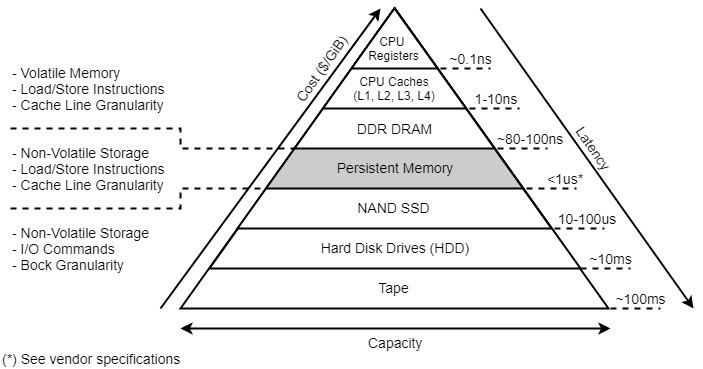
\includegraphics[scale=0.6]{images/pmem_storage_pyramid.jpg}
    \caption{Memory Hierarchy. Taken from \cite{Introduc86:online}}
    \label{fig:pmem_storage_pyramid}
\end{figure}

Persistent memory, also referred to as Non-Volatile Memory (NVM), represents a significant evolution in the memory/storage hierarchy (Figure \ref{fig:pmem_storage_pyramid}), addressing the performance and capacity gap between dynamic random-access memory (DRAM) and traditional storage mediums. This innovative technology combines the characteristics of both DRAM and storage, offering the speed of DRAM and the non-volatile nature of storage devices \cite{scargall2020pmem}.

Like DRAM, persistent memory is available in the form of Dual In-line Memory Modules (DIMMs), which are directly connected to the memory bus. This direct connection enables applications to access persistent memory with the same ease as traditional DRAM, eliminating the need for frequent data transfers between memory and storage. However, unlike DRAM, persistent memory DIMMs provide significantly greater capacity and retain data even when power is removed, thereby enhancing system performance and enabling fundamental changes in computing architecture \cite{rudoff2017persistent,scargall2020pmem}.

Intel Optane DC Persistent Memory Module (Optane PMM) stands at the forefront of commercial implementations of persistent memory technology, leveraging Intel's innovative 3D-XPoint technology. Upon its introduction, the Optane PMM offers substantial capacities up to 512GiB and is exclusively supported by Intel Cascade Lake platform. Each processor within this platform is equipped with two integrated memory controllers (iMCs), with each iMC supporting three channels. This architecture seamlessly integrates Optane PMM with DRAM, allowing users to deploy up to one Optane PMM per channel and up to six per CPU socket, thereby enabling extensive memory capacities of potentially up to 3TiB per socket \cite{yang2020empirical,izraelevitz2019basic}.

Similar to conventional DRAM DIMMs, Optane PMMs are positioned on the memory bus and connect directly to the processor's iMC. The communication protocol between the iMC and the Optane PMM is depicted in Figure \ref{fig:optane_communication}.  Communication between the iMC and the Optane PMM occurs via the DDR-T protocol, adapted for persistent memory and operating at cache line granularity (64B). Initial memory access to the Optane PMM is coordinated by the onboard Controller, which manages access to the 3D-XPoint media. Analogous to SSDs, the Optane PMM conducts address translation for wear-leveling and bad block management, facilitated by the maintenance of an address indirection table (AIT). Following translation, access to the storage media occurs. Notably, with 3D-XPoint access granularity set at 256B, the controller converts 64-byte accesses into 256-byte accesses, inducing write amplification. To mitigate this, the Controller incorporates a 16KB write-combining buffer to merge adjacent writes \cite{yang2020empirical,izraelevitz2019basic,wu2020ribbon}.

\begin{figure}[ht]
    \centering
    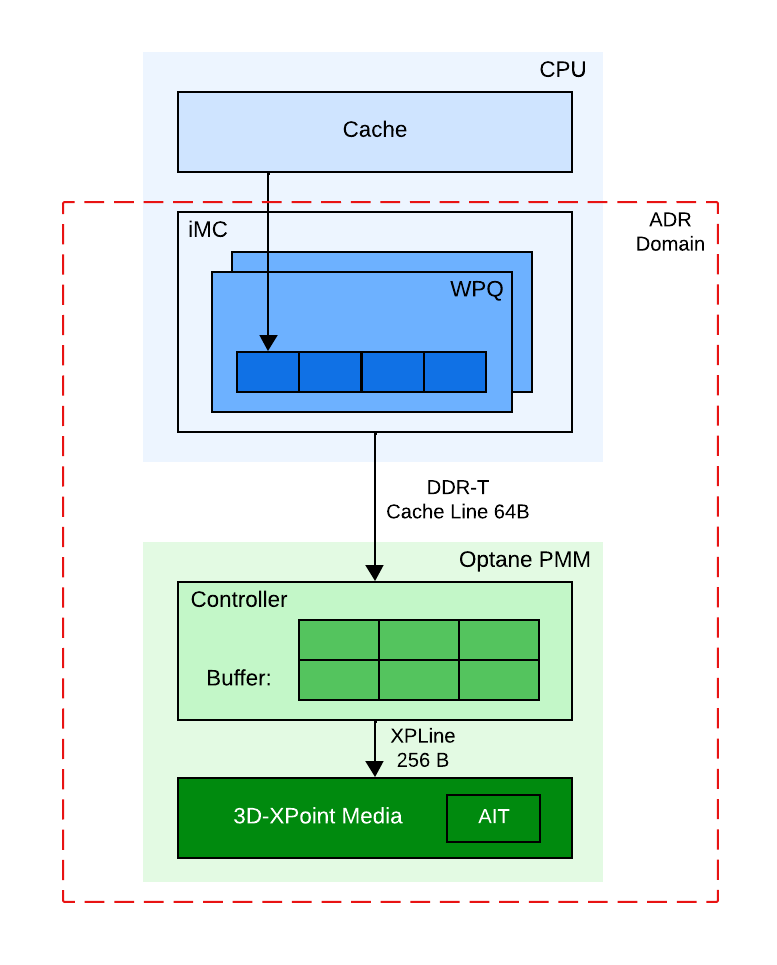
\includegraphics[scale=0.7]{images/optane-communication.png}
    \caption{Communication between iMC and Optane PMM}
    \label{fig:optane_communication}
\end{figure}

To ensure data persistence, Intel platforms integrate the iMC and Optane PMM within the asynchronous DRAM refresh (ADR) domain. Intel's ADR feature ensures that CPU stores that reach the ADR domain will survive a power failures \cite{yang2020empirical}. The iMC manages read and write pending queues for each Optane PMM, with the ADR domain encompassing the write pending queue. Once data reaches the write pending queue, ADR ensures its persistence within Optane PMM in the event of power failures. The ADR domain excludes the CPU caches, necessitating additional steps beyond simply executing a store instruction to ensure data persistence. To achieve this, CPU stores must be continually flushed using specialized instructions provided by Intel's Instruction Set Architecture (ISA), including \textrm{CLFLUSH}, \textrm{CLFLUSHOPT}, and \textrm{CLWB} \cite{yang2020empirical,izraelevitz2019basic,rudoff2017persistent}.

\subsection{Performance Characterization}
Previous studies \cite{yang2020empirical,izraelevitz2019basic} conducted an empirical performance assessment of Optane PMM, revealing its nuanced behavior compared to DRAM. They observed that Optane's performance varies significantly depending on specific access patterns, including access size, type, and concurrency level. Notably, they found that Optane's read latency is three times slower than that of DRAM, primarily due to Optane's longer media latency. However, sequential access patterns demonstrate notably improved latency, indicating Optane PMM's capability to consolidate adjacent requests into single 256-byte accesses. The study also highlights that Optane PMM achieves a maximum random read bandwidth of 6.6 GB/s and a write bandwidth of 2.3 GB/s. Moreover, sequential access further enhances bandwidth performance, exhibiting up to a fourfold increase \cite{yang2020empirical,izraelevitz2019basic}.

An insightful observation highlighted by Izraelevitz et al. \cite{izraelevitz2019basic} is that Optane PMM's bandwidth can become saturated when utilized in real-world multi-threaded applications, thereby introducing performance overhead. This phenomenon arises due to Optane PMM's inability to scale performance proportionally with increased thread count, primarily due to contention occurring within the processor's integrated memory controller (iMC) and Optane PMM's buffer. Contentious conditions within the buffer exacerbate the frequency of evictions and write-backs to the 3D-XPoint media, resulting in Optane writing more data internally than what the application necessitates. Furthermore, given Optane PMM's slightly slower performance compared to DRAM, the slower drainage of write pending queues by Optane PMMs introduces head-of-line blocking effects. As the number of threads concurrently accessing Optane PMM increases, contention on the device escalates, heightening the likelihood of the processor experiencing blocking while awaiting completion of previous store operations \cite{yang2020empirical}.

\subsection{Operating Modes and Applications}

Intel Optane persistent memory (PMem) offers two distinct operating modes: Memory mode and App Direct mode.

In Memory mode, Optane PMem serves as a high-capacity main memory without persistence. In this configuration, DRAM is concealed from users and acts solely as a cache for Optane PMem, seamlessly managed by the operating system \cite{yang2020empirical}. 

Conversely, in App Direct mode, Optane PMMs are directly exposed to the operating system as independent persistent memory devices, thus enabling their utilization for persistent storage \cite{izraelevitz2019basic}. Functionally, the operating system perceives DRAM and Optane PMem as distinct memory pools, with the latter offering data persistence. Applications can access Intel Optane persistent memory through direct load/store operations or via a file system configured with the \textrm{dax} (direct access) option. Such a file system is termed as a PM-aware file system, facilitating direct access to persistent memory without relying on the page cache \cite{rudoff2017persistent}.

In the context of this thesis, Optane PMem is exclusively employed in App Direct Mode, coupled with a PM-aware file system to harness its storage capabilities.

\subsection{Programming Persistent Memory}

In the realm of persistent memory technology, maintaining data consistency across runtime and system reboots is essential. To address this challenge, prior research underscores the necessity for applications leveraging persistent memory to implement transactions that are atomic, consistent, thread-safe, and resilient to system failures—a paradigm akin to ACID transactions in database systems. However, achieving such robustness in real-world scenarios poses significant complexity. Recognizing this, Intel has developed the Persistent Memory Development Kit (PMDK) to tackle this challenge \cite{scargall2020pmem,rudoff2017persistent}.

PMDK comprises a comprehensive suite of libraries and tools tailored for both application developers and system administrators, aiming to streamline the management and utilization of persistent memory devices. Drawing on the SNIA NVM Programming model \cite{NVMProgr73:online} as its foundation, these libraries extend its capabilities to varying extents. Some libraries offer simplified wrappers around operating system primitives, facilitating ease of use, while others provide sophisticated data structures optimized for persistent memory usage \cite{scargall2020pmem}.

In the scope of this thesis, we leverage pmemkv \cite{GitHubpm66:online}, a persistent local key-value store provided by PMDK. Designed with cloud environments in mind, pmemkv complements PMDK's suite of libraries with cloud-native support, abstracting the intricacies of programming with persistent memory through a familiar key-value API. Notably, pmemkv distinguishes itself from traditional key-value databases by enabling direct access to data. This means that reading data from persistent memory circumvents the need for copying it into DRAM—an approach that significantly enhances the performance of applications leveraging persistent memory \cite{scargall2020pmem}.

\section{Serverless Computing}

Serverless computing, a prominent execution model within cloud computing, revolutionizes the deployment process by allowing developers to deploy code without the need for provisioning or managing server infrastructure. Although termed "serverless," this model still utilizes servers provided by cloud vendors to execute developers' code. However, the distinguishing feature lies in the abstraction of infrastructure management from the developer's perspective. Developers no longer concern themselves with resource provisioning, scaling, fault tolerance, monitoring, or security patches; instead, they focus solely on code development. Cloud providers take on the responsibility of handling these infrastructure-related tasks on behalf of their customers. Consequently, developers are charged based on the execution time and resources consumed during their code invocations, offering a pay-per-use billing model \cite{jonas2019cloud,romero2021faat,klimovic2018pocket}.

At the heart of serverless computing lies Function-as-a-Service (FaaS), introduced by AWS Lambda in 2015. Since then, various commercial and open-source alternatives have emerged, including Google Cloud Functions, Azure Functions, Apache OpenWhisk, and others. FaaS enables developers to express application logic as stateless functions written in high-level languages such as Java, Python, C, or C++. These functions are packaged together with their dependencies and submitted to the serverless platform. Additionally, developers associate events with each function, such as HTTP requests, file uploads, database triggers, and more. Upon the occurrence of a trigger, the cloud provider promptly executes the associated function, offering a scalable and event-driven approach to application development and deployment \cite{AWSLambd40:online,AzureFun49:online,CloudFun3:online,ApacheOp28:online}.

\subsection{Storage for FaaS}



\section{Reinforcement Learning}

Reinforcement Learning (RL) is a subfield of machine learning concerned with learning optimal decision-making policies through interactions with an environment \cite{sutton2018reinforcement}. 

\subsection{Overview of Reinforcement Learning}
The fundamental concept underlying RL is the notion of an agent, which takes actions in an environment and receives feedback in the form of rewards, indicating the quality of its decisions. The agent's objective is to learn a policy that maximizes cumulative rewards over time. Moreover, the agent is not provided with explicit instructions on which actions to take; instead, it must discover the actions that lead to the highest rewards by trying them.

\begin{figure}[ht]
    \centering
    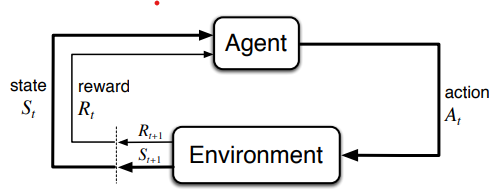
\includegraphics[scale=1]{images/rl-workflow.png}
    \caption{RL Workflow}
    \label{fig:sutton_rl_workflow}
\end{figure}

Figure \ref{fig:sutton_rl_workflow} presents a schematic representation of a standard reinforcement learning scenario. In discrete time steps, the agent perceives the current state $s_t$ from the set of all possible states $S$. It then selects an action $a_t$ from the available actions $A(s_t)$ in the current state. The environment transitions to a new state $s_{t+1}$, and the agent receives a reward $r_t$ associated with the transition $(s_t, a_t, s_{t+1})$.

The agent's behavior is governed by its policy, which maps perceived states to actions. The ultimate aim is to learn an optimal or near-optimal policy that maximizes the cumulative reward. 


\subsection{Q-Learning}

One of the foundational algorithms in RL is Q-Learning, introduced by Watkins in 1989 \cite{watkins1989learning}. The algorithm belongs to the class of model-free RL algorithms, meaning it learns directly from experience without requiring a model of the environment dynamics \cite{russel2020ai}.

At the core of Q-Learning is the Q-value function, denoted as $Q(s, a)$, which represents the expected cumulative reward the agent will receive by taking action $a$ in state $s$ and following an optimal policy thereafter. The objective of Q-Learning is to iteratively update the Q-values based on observed transitions and rewards, eventually converging to the optimal Q-values that maximize long-term rewards.

The Q-Learning algorithm proceeds as follows: the agent interacts with the environment by selecting actions based on its current estimate of the Q-values. Upon taking an action, the agent observes the resulting reward and the next state. It then updates the Q-value of the previous state-action pair using the observed reward and the estimated value of the next state.

The Q-value update rule in Q-Learning is based on the Bellman equation, which expresses the relationship between the Q-values of successive states \cite{russel2020ai}:

\[
Q(s, a) \leftarrow (1 - \alpha) \cdot Q(s, a) + \alpha \cdot \left( r + \gamma \cdot \max_{a'} Q(s', a') \right)
\]

Here, $\alpha$ is the learning rate, determining the extent to which new information overrides the old one, and $\gamma$ is the discount factor, representing the importance of future rewards relative to immediate rewards. The term $r + \gamma \cdot \max_{a'} Q(s', a')$ is known as the temporal-difference (TD) target, combining the immediate reward $r$ with the discounted maximum Q-value of the next state $s'$ \cite{russel2020ai}.

% Q-Learning, a model-free reinforcement learning algorithm, is employed by the agent to determine the best action given the current state. The agent evaluates action quality using a quality-function (Q-function) $Q(s, a)$, representing the expected total discounted reward if the agent selects action $a$ in state $s$ and acts optimally thereafter. 

% One of the foundational algorithms in RL is Q-Learning, introduced by Watkins in 1989 \cite{watkins1989learning}. Q-Learning is a model-free algorithm that learns the value of taking an action in a particular state, known as the Q-value, and iteratively refines these values through experience. The Q-value represents the expected cumulative reward the agent will receive by taking an action in a given state and following an optimal policy thereafter.

% The Q-Learning algorithm (illustrated in Figure \ref{algo:q_learning}) involves iterative updates to the Q-function. At each step, the agent selects an action, observes the reward and new state, and then applies one-step Q-learning. The update is governed by the Q-learning formula, where the learning rate ($\alpha$) determines the extent to which new information overrides old data. This learned Q-function approximates the optimal Q-function, irrespective of the policy being followed.

\subsection{Linear Regression Models in Reinforcement Learning}

One of the key advantages of Q-Learning is its simplicity and ease of implementation. It requires only a table to store the Q-values, making it computationally efficient for small state and action spaces. However, Q-Learning faces challenges in environments with large state spaces, as maintaining a lookup table becomes infeasible due to memory and computational constraints.

Function approximation is a fundamental technique in reinforcement learning (RL) aimed at approximating the Q-Value function when dealing with large state or action spaces where tabular representations become impractical \cite{russel2020ai}. This approach allows RL agents to generalize from observed states to unseen states, facilitating decision-making in unexplored regions of the state space.

In the context of RL, linear regression models are commonly used for function approximation \cite{sutton2018reinforcement}.  These models approximate the Q-value function by leveraging a weighted linear combination of features, with each feature capturing a distinct aspect of the state space. Employing gradient-descent methods, notably stochastic gradient descent, enables iterative refinement of the parameters governing the linear function, aimed at minimizing a predefined loss function. This iterative optimization process empowers the model to progressively enhance its predictive accuracy and capture intricate patterns within the state-action space.

Hyperparameter tuning is a critical aspect of training linear regression models in RL \cite{bergstra2012random}. Hyperparameters, such as the learning rate, regularization strength, and feature scaling, significantly impact the performance and convergence of the models. A systematic approach to hyperparameter tuning involves experimenting with different combinations of hyperparameters, evaluating the performance of the trained models on a validation set, and selecting the optimal hyperparameters based on predefined criteria, such as validation error or performance metrics \cite{russel2020ai}.

\subsection{Exploration-Exploitation Tradeoff}

The exploration-exploitation tradeoff poses a significant challenge in reinforcement learning \cite{sutton2018reinforcement}. The agent must strike a balance between exploring unfamiliar actions to gather information and exploiting known actions for immediate rewards. Finding this balance is crucial for effective learning and task performance, as the agent gradually favors actions with higher expected rewards.

One classic strategy for balancing exploration and exploitation is the epsilon-greedy (e-greedy) algorithm \cite{sutton2018reinforcement}. The e-greedy policy selects the action that maximizes the estimated value with probability $1 - \epsilon$ (exploitation) and selects a random action with probability $\epsilon$ (exploration). This approach ensures that the agent continues to explore the environment while gradually exploiting more rewarding actions as it gains knowledge.

Decayed e-greedy methods aim to strike a balance between exploration and exploitation by gradually reducing the exploration rate $\epsilon$ as the agent gains more experience or as the training progresses \cite{sutton2018reinforcement}. This decay encourages the agent to explore the environment more extensively in the early stages of learning while gradually shifting towards exploitation as it becomes more knowledgeable.

\subsection{Reward shaping}

Reward shaping is a technique in reinforcement learning (RL) aimed at accelerating learning by modifying the reward signal provided to the agent. Traditional RL algorithms rely solely on sparse reward signals, which can make learning slow and inefficient, especially in complex environments. Reward shaping addresses this issue by providing additional, shaped rewards that guide the agent towards desirable behaviors. These shaped rewards are designed to provide more informative feedback to the agent, encouraging it to explore the state-action space more effectively. However, reward shaping must be carefully designed to avoid unintended consequences such as overfitting to the shaped rewards or incentivizing undesirable behaviors \cite{russel2020ai}.

\chapter[Optimizing Optane PMem Performance for Serverless Storage]{Optimizing Optane PMem Performance for Serverless Storage}

As discussed earlier, the introduction of Optane PMem presents a significant opportunity for serverless storage services. This memory technology offers a unique combination of cost-effective high capacity, high performance, and support for data persistence \cite{IntelOp15:online}. When utilized in App-Direct mode, Optane PMem DIMMs and DRAM DIMMs function as independent memory resources directly controlled by applications for load/store operations. This configuration allows Optane PMem capacity to serve as byte-addressable persistent memory mapped into the system application space, providing direct accessibility to applications. Consequently, Optane PMem can function as persistent storage with memory-like speeds.

However, resource contention within Optane PMem can lead to substantial performance and contractual implications for multi-tenant serverless storage services. The limited capability of Optane PMem to handle accesses from multiple threads can result in degraded system performance during workload spikes, undermining the hallmark autoscaling features of serverless computing. Moreover, in multi-user environments, where physical resources are shared among tenants, performance variations due to Optane PMem contention can hinder service providers from offering consistent service level agreements.

To mitigate contention effects, prior research recommends restricting the number of threads accessing Optane PMem simultaneously. For instance, Yang et al. \cite{yang2020empirical} enhanced the performance of an PM-aware file system by limiting the number of writer threads accessing each Optane PMem DIMM. Similarly, Ribbon \cite{wu2020ribbon} dynamically adjusts the number of threads performing cache line flushing (CLF) operations at runtime. While effective, such approaches introduce management complexities for system administrators managing multi-tenant serverless storage environments.

Given the intricate nature of FaaS workloads, implementing efficient concurrency control mechanisms to optimize an Optane PMem-based serverless storage service is challenging. These challenges are elaborated in Section 3.1, but, in summary, service providers face three key tasks: ensuring predictable performance to meet diverse SLAs, transparently scaling resources to match current workload demands, and swiftly adapting to sudden workload shifts. To address these challenges, we propose a solution that shoulders these responsibilities on behalf of service providers.

This chapter introduces the NVM Middleware, a middleware optimization layer positioned between a serverless storage service and Intel Optane PMem. Its primary objective is to address the limitations associated with Optane PMem while simultaneously meeting the diverse (SLAs) required by multiple tenants amid varying workloads. Additionally, the chapter describes the development of a reinforcement learning agent to enable the NVM Middleware to quickly adapt to changing workloads. This agent considers workload characteristics and SLAs metrics, learning from past experiences to dynamically scale resources.
% The NVM Middleware distinguishes between latency-critical and throughput-oriented workloads, employing tailored concurrency control mechanisms for each category. This approach minimizes contention on the memory device and reduces interference among workloads with differing SLAs. Additionally, we propose the development of a reinforcement learning agent to enable the NVM Middleware to quickly adapt to changing workloads. This agent considers workload characteristics and SLAs, learning from past experiences to dynamically scale resources.

The subsequent sections of this chapter elaborate on the design objectives of the NVM Middleware, providing insights into its architectural principles and programming interface. Furthermore, the chapter delves into the implementation aspects of the reinforcement learning model, elucidating the training methodology employed to equip an agent with the capability to dynamically adjust the NVM Middleware's concurrency levels in response to fluctuating workloads. Lastly, the chapter provides an in-depth discussion on the implementation intricacies of the NVM Middleware.

\section{Motivation}

In this section, we discuss the pain points of controlling concurrency levels to optimize Optane PMem within a serverless storage service and explain the design goals of the NVM Middleware.

\subsection{Concurrency Control Challenges in Serverless Storage}

When building an Optane PMem-based serverless storage service, optimizing the memory's performance is just the start. Early works in serverless computing have identified several tasks that a storage service must perform efficiently to meet the demands of serverless computing \cite{180275,jonas2019cloud,klimovic2018understanding,klimovic2018pocket,wu2019autoscaling,romero2021faat}. As a result, service providers must ensure that their concurrency control policies do not interfere with these design goals. In this work, we focus on three challenges faced by service providers when designing a high-performance storage service.

\subsubsection{Support for a wide heterogeneity of applications}

In serverless computing, applications are often deployed as a set of serverless functions that interact with remote storage for data sharing. Previous research indicates significant diversity among these applications concerning data access size \cite{klimovic2018pocket,romero2021faat}, access patterns \cite{romero2021faat}, and performance requirements \cite{180275,jonas2019cloud}. Consequently, service providers encounter the challenge of adjusting concurrency levels to accommodate various application types. In this study, we focus on two distinct application categories: interactive applications, which prioritize low-access latency, and batch applications, which emphasize achieving high throughput.

% In this work, we argue that considering the workload characteristics is key for tuning the system efficiently. The allocation of resources can vary depending on the workload type.

\begin{figure}[ht]
  \centering
  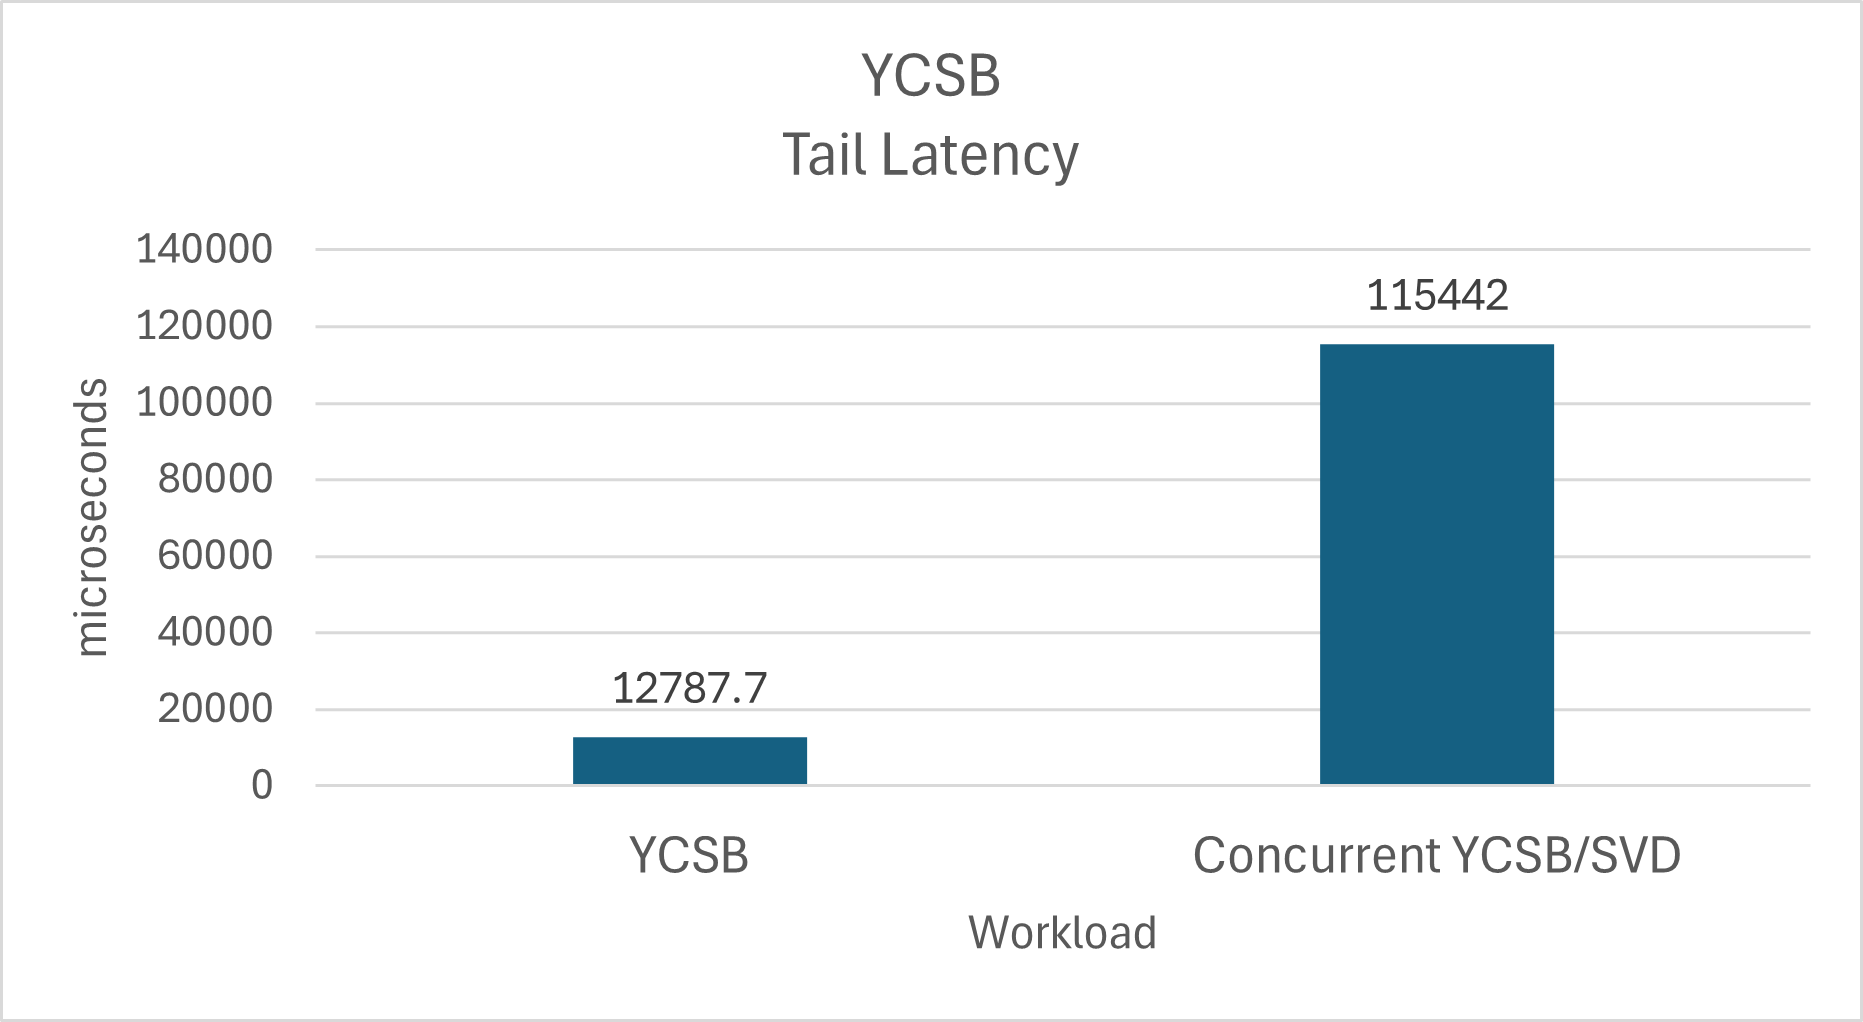
\includegraphics[width=0.7\textwidth,height=\textheight,keepaspectratio,angle=0]{images/measurement-study-latency.png}
  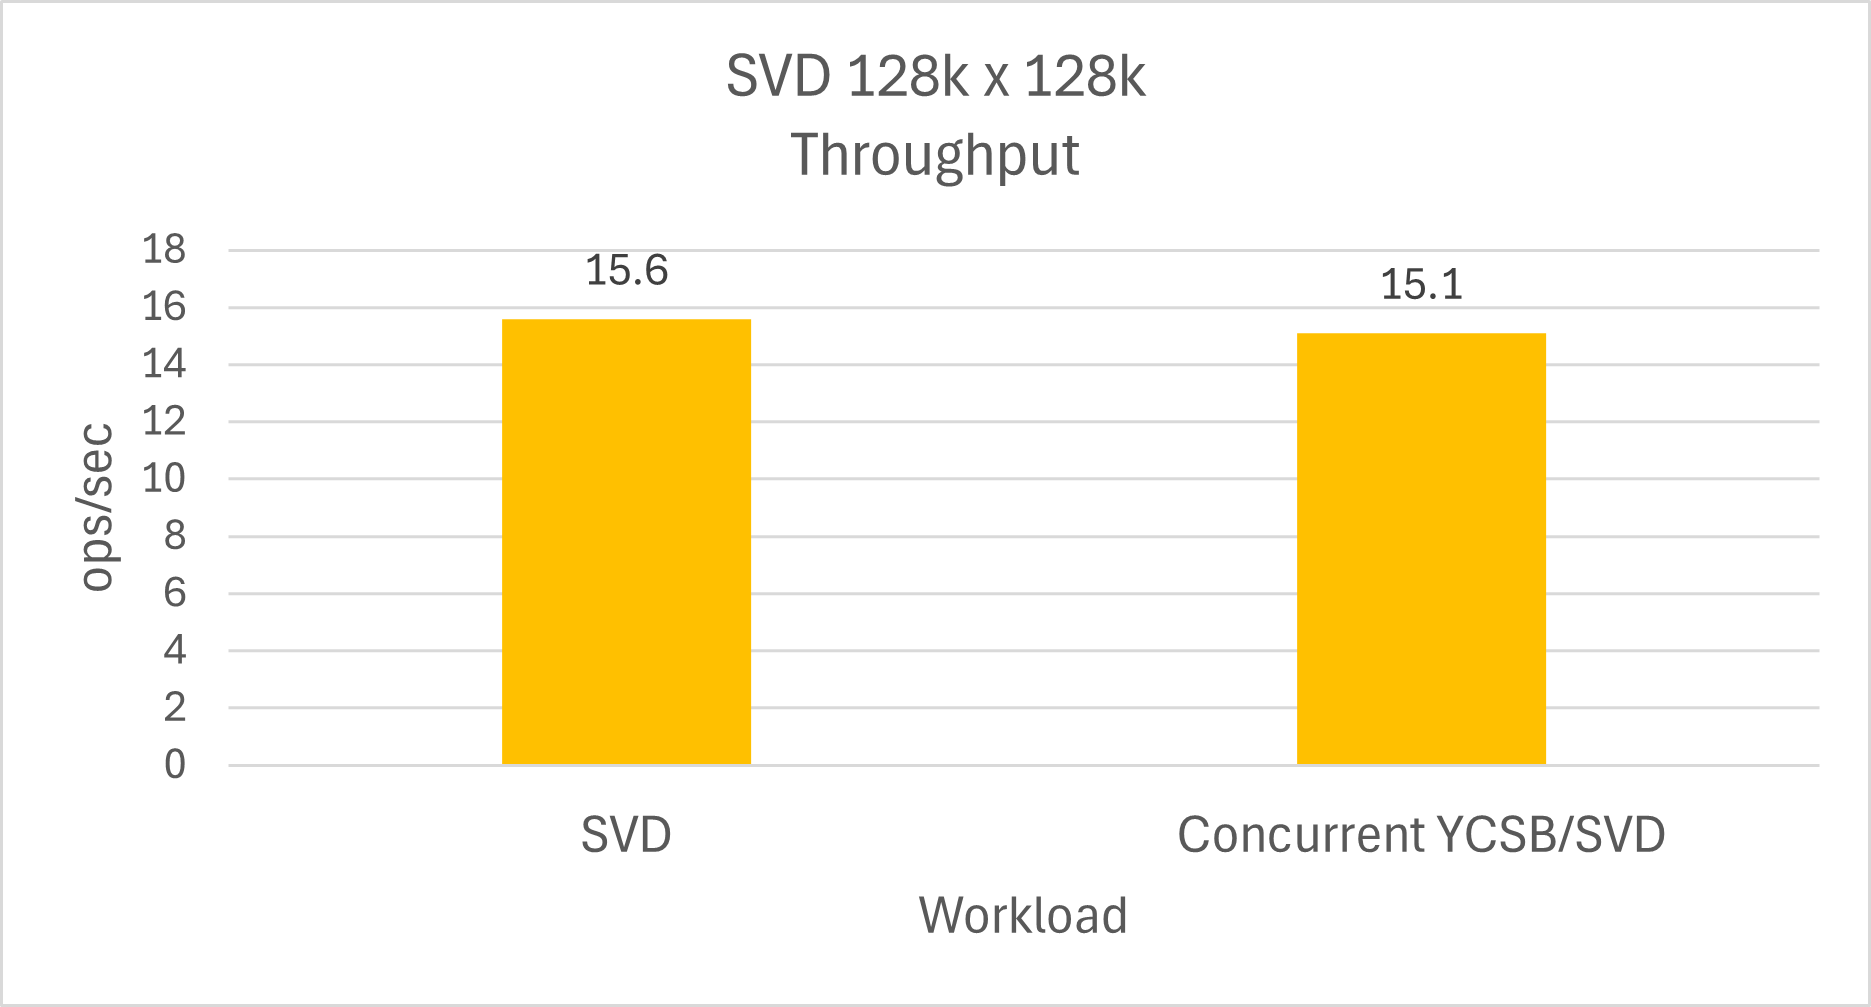
\includegraphics[width=0.7\textwidth,height=\textheight,keepaspectratio,angle=0]{images/measurement-study-tp.png}
  \caption[Impact of Concurrent Applications on Optane PMem 99th Latency and Throughput]{Comparison of 99th latency and throughput variations observed in Optane DC PMem when running YCSB and SVD applications concurrently. The top image depicts the latency comparison between YCSB running alone and concurrently with SVD, while the bottom image illustrates the throughput comparison between SVD running alone and concurrently with YCSB. Notably, concurrent application execution significantly impacts the 99th latency compared to throughput.}
  \label{fig:measurement_study}
\end{figure}

A measurement study was conducted to evaluate the effects of concurrent interactive and batch applications sharing Optane PMem. The study utilized the applications and experimental platform detailed in Section 4. The results are illustrated in Figure \ref{fig:measurement_study}. In this experiment, both an interactive application (YCSB) and a batch application (SVD) were executed individually and concurrently, utilizing Optane PMem as their storage medium. The findings illustrate a noticeable impact on both throughput and 99th latency when running the applications concurrently. Particularly, latency is significantly affected compared to throughput, suggesting contention among tenant workloads sharing Optane PMem. Hence, effective concurrency control mechanisms are essential to mitigate such contention, while reaching a balance between latency and throughput exhibited.

\subsubsection{Compliance with Service Level Agreements}

The success of a storage service relies on its ability to comply with various SLAs. SLAs play a critical role in governing the relationship between the storage provider and its customers. They help establish clear expectations between both parties regarding the quality of storage service. Therefore, service providers face the challenge of staying in compliance with these SLAs while they seek to optimize Optane PMem. 

\subsubsection{Automatic and transparent scaling}

Serverless workloads are extremely unpredictable. These workloads can launch hundreds of functions instantaneously to meet application demands \cite{klimovic2018understanding}. Furthermore, the data access patterns of the applications can change dramatically over time \cite{romero2021faat,wu2019autoscaling}. Service providers face the challenge of scaling the resources, such as number of threads, automatically to meet the demands of changing workloads. In addition, they must ensure that the system adapts quickly enough to avoid missing SLAs.

\subsection{NVM Middleware Design Overview}

We design NVM Middleware with two main design goals.

\textbf{Workload-aware Contention Management.} The NVM Middleware leverage insights about the workload characteristics and performance requirements of applications to make informed decisions about resource allocation and contention resolution. It dynamically adjusts resource allocation for each application type independently, mitigating performance degradation caused by contention and enabling efficient resource sharing among co-located applications.. This adaptive approach enables the NVM Middleware to allocate resources judiciously to maximize overall system efficiency and meet diverse performance requirements of both interactive and batch applications. By using the workload-aware contention management offered by the NVM Middleware, a storage system using Optane PMem can effectively balance the needs of different workload types, ensuring optimal performance and fair share of resources.

\textbf{RL-driven autoscaling policies.} Our solution proposes the use of Reinforcement Learning to dynamically scale resources, learning from historical data and anticipating changes in workload patterns. By incorporating information from SLAs to guide the learning process, the NVM Middleware can quickly adapt to changing worload patterns over time and meet SLA objectives more effectively than traditional threshold-based approaches \cite{cano2017curator}. Moreover, given the dynamic and unpredictable nature of FaaS workloads, we propose a model-free algorithm, Q-Learning, to continuously learn the optimal policy based on observed experiences, allowing the NVM Middleware to adapt to new scenarios without needing to explicitly model them.

\section{NVM Middleware Architecture}

\begin{figure}[ht]
  \centering
  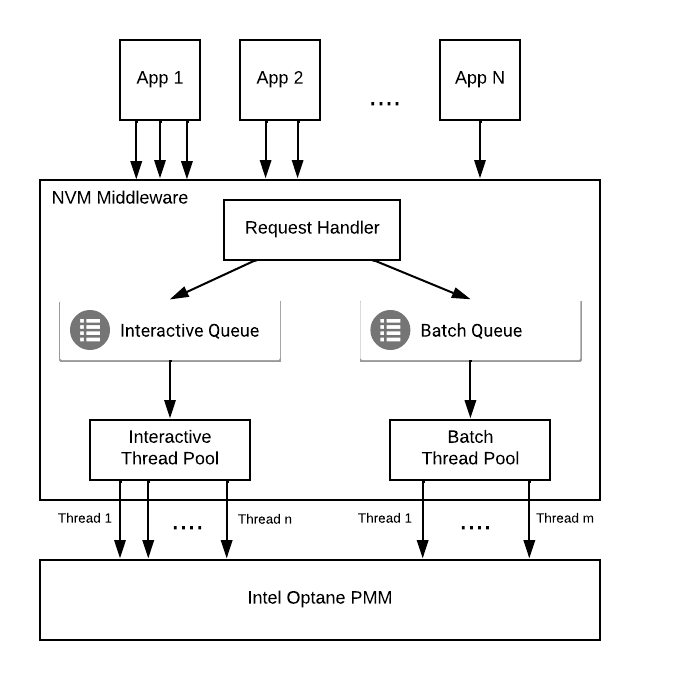
\includegraphics[scale=1]{images/nvm_design.png}
  \caption[NVM Middleware Architecture]{Illustration depicting the architecture of the NVM Middleware, which serves as an optimization layer for Optane PMem. The NVM Middleware governs the concurrency level on the device, categorizing incoming I/O requests based on their type (blue for interactive and orange for batch) and assigning distinct worker threads for interactive or batch workloads. The number of threads for each workload type is dynamically configurable to adapt to the system's requirements.}
  \label{fig:nvm_architecture}
\end{figure}

Figure \ref{fig:nvm_architecture} provides an overview of the NVM Middleware architecture. Positioned as a middle layer connecting user applications with Optane PMem, its design is tailored for seamless integration within a storage service, serving as an optimization layer specifically targeting Optane PMem. It comprises a request handler, two concurrency thread pools, and a monitoring and resource management module.

The request handler serves as the primary interface for handling user I/O requests. Upon receipt, it segregates requests into two distinct non-blocking First-In-First-Out (FIFO) queues: one tailed for interactive requests and the other for batch ones. Leveraging insights into workload characteristics, the handler intelligently allocates requests to the appropriate queue. Moreover, each queue is assigned a dedicated pool of worker threads tasked with dispatching I/O requests to Optane PMem using PMEMKV. These worker threads are categorized as either interactive or batch threads. Notably, these thread pools operate independently and are dynamically managed and scaled by the Reinforcement Learning agent to meet predetermined latency and throughput goals.

The Monitoring and Resource Management module offers an interface to monitor system load and SLA performance metrics. This module initiates a separate control thread tasked with gathering data on key parameters within the NVM Middleware, such as 99th latency, throughput, and system load. Utilizing this information, the RL agent makes data-driven decisions regarding optimal thread pool scaling. Subsequently, these decisions are communicated to the Monitoring and Resource Management module, which executes the required actions within the NVM Middleware.

\section{NVM Middleware Programming Interface}

\begin{table}[ht]
  \centering
  % \caption[NVM Middleware Programming Interface]{Overview of the NVM Middleware programming interface, categorized by functionality. $System$ functions facilitate resource management within the middleware, including database initialization and thread pool management. $Storage$ functions provide a fundamental key-value interface for submitting requests aimed at accessing persistent memory. $RL$ functions provide utilities for the reinforcement learning process, enabling monitoring of system statistics, state retrieval, and triggering scaling actions.}
  \caption[NVM Middleware Programming Interface]{Overview of the NVM Middleware programming interface, categorized by functionality. $System$ functions facilitate resource management within the NVM Middleware, including database initialization and thread pool management. $Storage$ functions provide a fundamental key-value interface for submitting requests aimed at accessing persistent memory. $RL$ functions provide utilities for the reinforcement learning process, enabling monitoring of system statistics, state retrieval, and triggering scaling actions.}
  \label{table:programming_interface}
  % Tabular environment goes AFTER the caption!
  \begin{adjustbox}{width=1\textwidth}
  \begin{tabular}{|l|l|l|}
    % after \\: \hline or \cline{col1-col2} \cline{col3-col4} ...
    \hline
    \thead{Category} & \thead{API Name} & \thead{Functionality} \\
    \hline
    System & start(db, interactiveThreads, batchThreads) & \makecell[cl]{Create the PMEMKV database, start thread pools, \\ and initiate NVM Middleware's monitoring.} \\
    \hline
    System & stop() & \makecell[cl]{Close PMEMKV database, stop thread pools, \\ and stop NVM Middleware's monitoring.} \\
    \hline
    Storage & get(key, mode) & \makecell[cl] {Submits request to retrieve a key from \\ persistent memory.} \\
    \hline
    Storage & put(key, value, mode) & \makecell[cl] {Submits request to write a key to \\ persistent memory.} \\
    \hline
    RL & get\_stats() & \makecell[cl] {Provides the 99th percentile and throughput \\ observed by the NVM Middleware.} \\
    \hline
    RL & get\_state() & \makecell[cl] {Provides the current state within the \\ NVM Middleware.} \\
    \hline
    RL & perform\_action(action) & Triggers a scaling action. \\
    \hline
  \end{tabular}
\end{adjustbox}
\end{table}


Table \ref{table:programming_interface} outlines the NVM Middleware's programming interface, presenting a set of functions designed to facilitate interaction with a storage system and the reinforcement learning agent. 

The $start$ function initializes the PMEMKV database, initializes the thread pools with an initial thread count, and triggers the system monitoring within the Monitoring and Resource Management Module. In contrast, the $stop$ function terminates the database connection, halts all threads in the thread pools, and stops system monitoring. Furthermore, the $get$ and $put$ functions facilitate key-value interactions with the persistent memory, allowing for read and write operations. These functions are designed to accommodate hints regarding the request type (e.g., latency-sensitive or throughput-oriented), aiding the request handler in queue allocation.

The $get\_stats$ function furnishes insights into the 99th percentile and throughput observed by the NVM Middleware at any given moment. Similarly, the $get\_state$ function provides real-time state information as outlined in Table \ref{table:state_space}. Finally, the $perform\_action$ function accepts scaling actions detailed in Table \ref{table:action_space} and initiates the corresponding action within the NVM Middleware.

\section{Reinforcement Learning Component}

In this section, we discuss the Q-learning algorithm used by the RL agent to dynamically adjust the number of threads assigned to each thread pool. The agent’s goal is to find the best combination of threads that meets predetermined latency and throughput SLAs while minimizing contention and ensuring efficient utilization of Optane PMem. 

\subsection{Integration with the NVM Middleware}

\begin{figure}[ht]
  \centering
  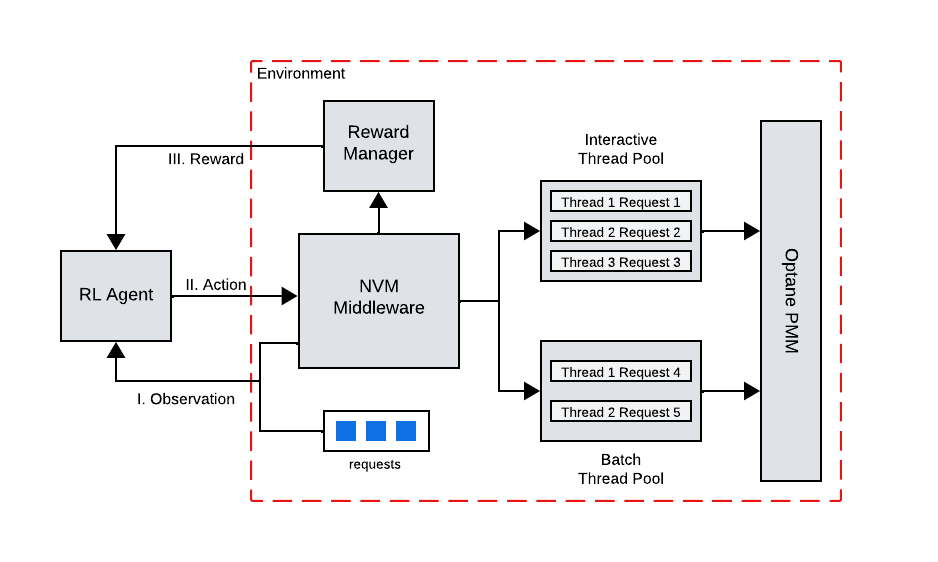
\includegraphics[scale=1]{images/rl_workflow.png}
  \caption[Interaction between Reinforcement Learning Agent and NVM Middleware]{Interaction between the RL agent and the NVM Middleware. At each time step, the RL agent observes (I) the state of the environment and takes a scaling action (II) on the NVM Middleware based on its learned policy. Subsequently, the agent receives a reward (III), which is utilized to iteratively refine its policy.}
  \label{fig:rl_workflow}
\end{figure}

Figure \ref{fig:rl_workflow} offers a visual representation of the interaction between the RL agent and the NVM Middleware. At each time step, the NVM Middleware receives a diverse influx of requests, spanning both interactive and batch tasks. These requests necessitate translation into actionable I/O commands directed towards the Optane PMem.

Concurrently, the RL agent adeptly captures the environment's current state, leveraging real-time workloads' characteristics and performance metrics provided by the monitoring module. Utilizing this information, the agent orchestrates the selection of an optimal action, guiding the dynamic adjustment of threads within the interactive and batch thread pools. This adaptive decision-making process is exemplified by actions like augmenting the count of interactive threads to address evolving workload demands.

Following action selection, the NVM Middleware's resource management module implements the chosen course of action, fine-tuning the NVM Middleware's interactive and batch threads to efficiently handle incoming user requests. Upon the completion of each time step, the action's effectiveness is rigorously assessed against predefined SLA targets, yielding a reward signal generated by a reward manager.

The reward serves as invaluable feedback for the RL agent, empowering iterative policy updates aimed at refining decision-making strategies in subsequent time steps. Thus, the presented framework embodies a recursive learning cycle, wherein the RL agent continuously hones its behavior through real-world interactions, ensuring adaptive responsiveness to evolving workload dynamics.

\subsection{Reinforcement Learning Model}

\subsubsection{State Space}

\begin{table}[ht]
  \centering
  \caption[Reinforcement Learning State Representation]{State representation for the reinforcement learning model. The number of interactive and batch threads is capped at 32, as measurements showed performance degradation with more than 32 threads. The interactiveQueueSize and batchQueueSize represent the number of requests in the respective queues within the NVM Middleware. The block sizes and write ratios are determined by analyzing the I/O requests received from client workloads.}
  \label{table:state_space}
  \begin{adjustbox}{width=1\textwidth}
  \begin{tabular}{|l|l|l|}
    \hline
    \thead{Name} & \thead{Description} & \thead{Values} \\
    \hline
    interactiveThreads & \makecell[l]{Number of interactive threads assigned\\ to the interactive thread pool.} & $1 \leq \text{interactiveThreads} \leq 32$ \\
    \hline
    batchThreads & \makecell[l]{Number of batch threads assigned\\ to the batch thread pool.} & $1 \leq \text{batchThreads} \leq 32$ \\
    \hline
    interactiveQueueSize & \makecell[l]{Number of requests in the interactive queue.} & $\text{interactiveQueueSize} \in \mathbb{R}^+$ \\
    \hline
    batchQueueSize & \makecell[l]{Number of requests in the batch queue.} & $\text{batchQueueSize} \in \mathbb{R}^+$ \\
    \hline
    interactiveBlockSize & \makecell[l]{Average data access size of interactive workload.} & $\text{interactiveBlockSize} \in \mathbb{R}^+$ \\
    \hline
    batchBlockSize & \makecell[l]{Average data access size of batch workload.} & $\text{batchBlockSize} \in \mathbb{R}^+$ \\
    \hline
    interactiveWriteRatio & \makecell[l]{Proportion of write requests compared\\ to read requests in the interactive workload.} & $\text{interactiveWRatio} \in \mathbb{R}^+$ \\
    \hline
    batchWriteRatio & \makecell[l]{Proportion of write requests compared\\ to read requests in the batch workload.} & $\text{batchWRatio} \in \mathbb{R}^+$ \\
    \hline
  \end{tabular}
  \end{adjustbox}
\end{table}

Table \ref{table:state_space} presents the features of our state representation. At each time step $t$, we define the state $s_t$ as a tuple:

\[
\begin{aligned}
s_t = (& \text{interactiveThreads}_t, \text{batchThreads}_t, \text{InteractiveQueueSize}_t, \text{batchQueueSize}_t, \\
& \text{interactiveBlockSize}_t, \text{batchBlockSize}_t, \text{interactiveWRatio}_t, \text{batchWRatio}_t )
\end{aligned}
\]

where $s_t \in S$ represents the state space. The tuple encapsulates the key features characterizing the system's current state, including the number of interactive and batch threads, number of pending requests in the NVM Middleware's queues, individual workload data access sizes, and write ratio for both interactive and batch workloads.

\subsubsection{Action Space}

\begin{table}[ht]
  \centering
  \caption[Reinforcement Learning Action Space]{Possible actions in the action space of reinforcement learning and their effects on the NVM Middleware's concurrency control mechanism.}
  \label{table:action_space}
  \begin{tabular}{|c|l|l|}
  \hline
  \thead{Action} & \thead{Effect on \ Interactive Threads} & \thead{Effect on \ Batch Threads} \\
  \hline
  0 & No change & No change \\
  1 & Increase by 1 & No change \\
  2 & Decrease by 1 & No change \\
  3 & No change & Increase by 1 \\
  4 & No change & Decrease by 1 \\
  5 & Increase by 1 & Increase by 1 \\
  6 & Increase by 1 & Decrease by 1 \\
  7 & Decrease by 1 & Increase by 1 \\
  8 & Decrease by 1 & Decrease by 1 \\
  \hline
  \end{tabular}
\end{table}

  Table \ref{table:action_space} illustrates the feasible actions within the action space. Each action corresponds to a potential adjustment in the number of interactive and batch threads. The table enumerates nine distinct actions, each with its respective effect on the number of interactive threads and batch threads.

  Mathematically, the set of actions $A$ is defined as $A = \{0,1,2,3,4,5,6,7,8\}$ for a given state $s_t \in S$.

\subsubsection{Reward}

To guide the optimization process of the reinforcement learning agent, we establish an algorithm (Algorithm \ref{algo:reward_calculation}) to calculate a reward value based on observed and target latency and throughput metrics. This algorithm, outlined below, serves as a crucial component in training the RL agent to make informed decisions.

\begin{enumerate}
  \item Lines 1-5 define goals, scaling factors, and penalties. The observed and target latency ($lat$, $lat\_goal$) and throughput ($tp$, $tp\_goal$) metrics are scaled to a normalized range using scaling factors ($max\_scale\_lat$, $max\_scale\_tp$) and minimum scale ($min\_scale$). This normalization process ensures that both metrics contribute proportionally to the reward calculation.
  \item Lines 6-7 compare the scaled latency ($lat$) and throughput ($tp$) metrics against the scaled target values for latency ($lat\_goal$) and throughput ($tp\_goal$). The absolute differences between observed and target values are computed to quantify the error in latency ($error\_lat$) and throughput ($error\_tp$).
  \item Lines 8-12 determine the reward based on three distinct scenarios. Firstly, if both latency and throughput goals are achieved, a high positive reward is assigned. Secondly, if both goals are not met, a low negative reward is assigned, taking into account both latency and throughput errors. The disparity in penalties, represented by $lat\_penalty$ and $tp\_penalty$, ensures that both types of errors contribute proportionately to the overall reward. Thirdly, if only the latency goal remains unmet, a low negative reward is assigned, incorporating the latency penalty and error. Finally, if only the throughput goal is unmet, a similar low negative reward is assigned, encompassing the throughput penalty and error.
\end{enumerate}

\begin{algorithm}
  \small
  \caption{Reward Calculation Algorithm}
  \label{algo:reward_calculation}
  \SetAlgoLined
  \KwIn{System statistics: $\text{stat}$}
  \KwOut{Reward value: $\text{reward}$}
  \tcc{Initialize variables}
  $\text{max\_scale\_lat} \leftarrow 1000$, $\text{max\_scale\_tp} \leftarrow 10$, $\text{min\_scale} \leftarrow 1$, $\text{lat\_goal} \leftarrow 200$, $\text{tp\_goal} \leftarrow 250000$, $\text{lat\_penalty} \leftarrow 500.0$, $\text{tp\_penalty} \leftarrow 5000.0$\;
    
  \tcc{Scale observed and target latency and throughput}
  $\text{lat} \leftarrow ((\text{max\_scale\_lat} - \text{min\_scale}) \times (\text{stat.tailLatency} - \text{min\_value}) / (\text{max\_latency} - \text{min\_value})) + \text{min\_scale}$\;
  $\text{tp} \leftarrow ((\text{max\_scale\_tp} - \text{min\_scale}) \times (\text{stat.throughput} - \text{min\_value}) / (\text{max\_throughput} - \text{min\_value})) + \text{min\_scale}$\;
  $\text{lat\_goal} \leftarrow ((\text{max\_scale\_lat} - \text{min\_scale}) \times (\text{lat\_goal} - \text{min\_value}) / (\text{max\_latency} - \text{min\_value})) + \text{min\_scale}$\;
  $\text{tp\_goal} \leftarrow ((\text{max\_scale\_tp} - \text{min\_scale}) \times (\text{tp\_goal} - \text{min\_value}) / (\text{max\_throughput} - \text{min\_value})) + \text{min\_scale}$\;
    
  \tcc{Calculate errors}
  $\text{error\_lat} \leftarrow |\text{lat} - \text{lat\_goal}|$\;
  $\text{error\_tp} \leftarrow |\text{tp} - \text{tp\_goal}|$\;
    
  \tcc{Calculate reward}
  \eIf{$\text{lat} \leq \text{lat\_goal}$ \textbf{and} $\text{tp} \geq \text{tp\_goal}$}{
      $\text{reward} \leftarrow 10 \times (\text{error\_lat} + \text{error\_tp}$) \tcp*{High reward for meeting both latency and throughput goals}
  }{
      \eIf{$\text{lat} > \text{lat\_goal}$ \textbf{and} $\text{tp} < \text{tp\_goal}$}{
          $\text{reward} \leftarrow -1 \times (\text{lat\_penalty} \times \text{error\_lat} + \text{tp\_penalty} \times \text{error\_tp})$ \tcp*{Penalize for high latency and low throughput}
      }{
          \eIf{$\text{lat} > \text{lat\_goal}$}{
              $\text{reward} \leftarrow -1 \times \text{lat\_penalty} \times \text{error\_lat}$ \tcp*{Penalize for high latency}
          }{
              $\text{reward} \leftarrow -1 \times \text{tp\_penalty} \times \text{error\_tp}$ \tcp*{Penalize for low throughput}
          }
      }
  }
\end{algorithm}

\subsection{Training Methodology}

\subsubsection{Environment Design}

\begin{figure}[ht]
  \centering
  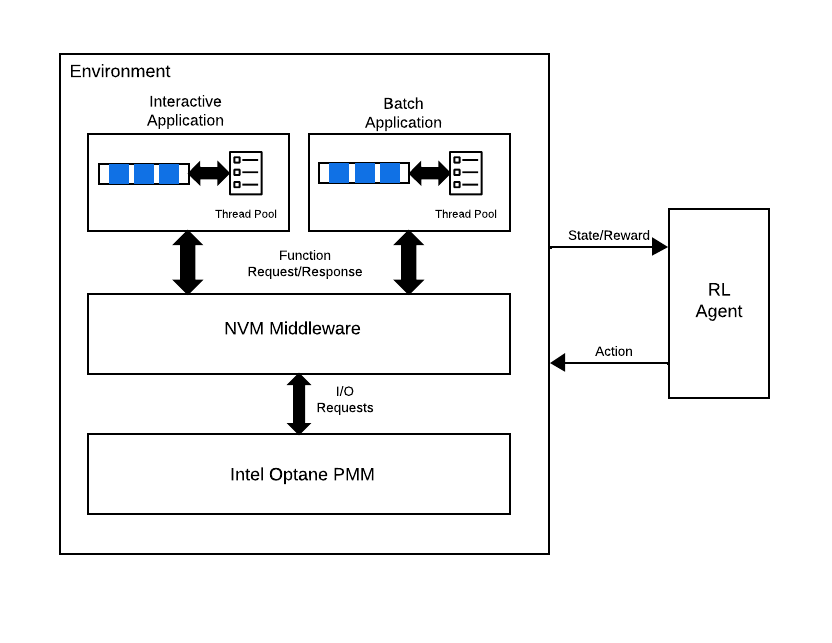
\includegraphics[width=1\textwidth]{images/rl_environment_architecture.png}
  \caption[Overview of the Reinforcement Learning Environment]{Overview of the RL environment constructed for training the RL agent. The environment employs multi-threaded interactive and batch applications to replicate workloads generated by multiple serverless functions with shared access to persistent memory. These applications interact with the NVM Middleware through function calls using its programming interface. Meanwhile, in the background, the agent continuously iterates through a closed feedback loop, observing the environment's state and executing scaling actions based on its policy.}
  \label{fig:rl_environment_architecture}
\end{figure}

The environment architecture designed for training and evaluating the RL agent is depicted in Figure \ref{fig:rl_environment_architecture}. This architecture comprises several key components, including an interactive multi-threaded application, a batch multi-threaded application, the NVM Middleware, and Intel Optane PMem.

To simulate a multi-tenant serverless scenario, both applications are executed concurrently. Workload patterns for each application are derived from collected serverless traces. To emulate high concurrency levels typical in serverless environments, multiple threads within each application are employed to dispatch requests to the NVM Middleware via the API described in Section 3.3. Meanwhile, the NVM Middleware processes these requests in accordance with the workflow outlined in Section 3.2.

\begin{figure}[ht]
  \centering
  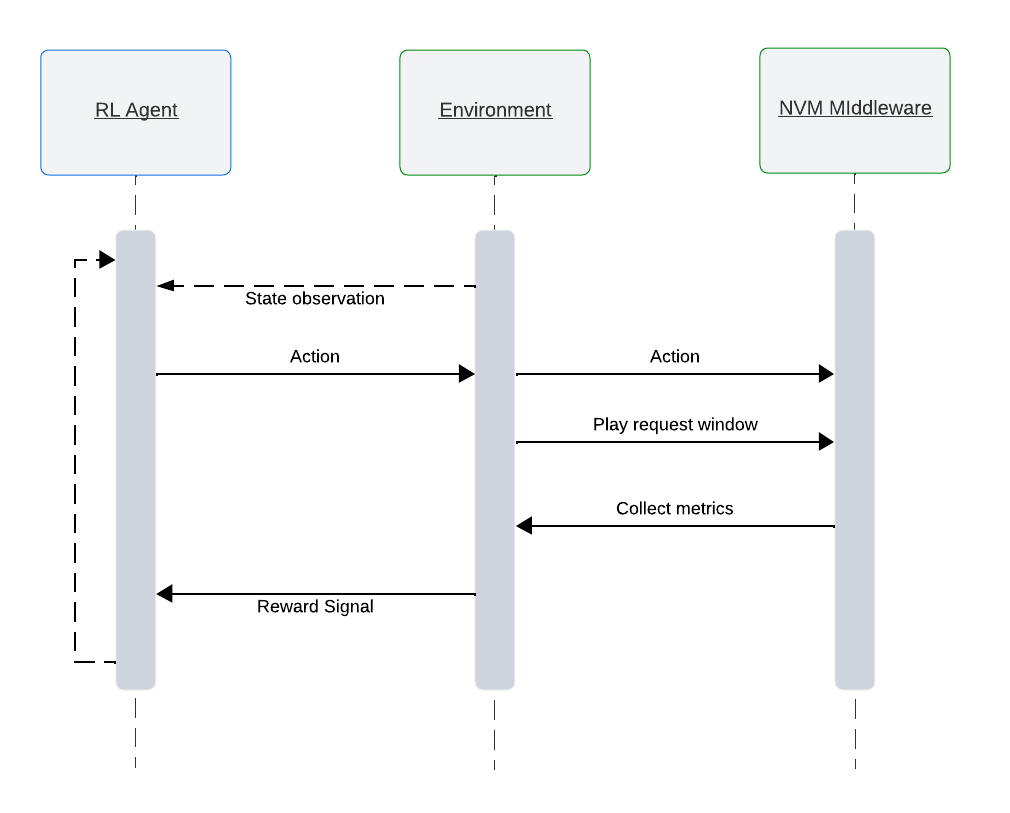
\includegraphics[width=1\textwidth]{images/rl_sequence_flow.png}
  % \caption[Reinforcement Learning Agent Process flow]{Illustration depicting the interaction between RL agent and its environment at each time step. At each time step, the agent's scaling action is performed before executing the next one-second window of I/O requests. Then the environment collects latency and throughput metrics to evaluate the action's efficiency and uses these metrics to return a reward signal that is used by the agent to improve its policy.}
  \caption[Reinforcement Learning Agent Process Flow]{Illustration depicting the interaction between the RL agent and its environment at each time step. During each time step, the agent executes a scaling action, followed by the processing of the subsequent window of I/O requests by the environment. Subsequently, the environment gathers latency and throughput metrics to assess the effectiveness of the action, providing a reward signal that the agent utilizes to refine its policy.}
  \label{fig:rl_sequence_flow}
\end{figure}

In order to model the time steps inherent in an RL process, the environment organizes the applications' requests into 1-second windows, processing one window per time step. Figure \ref{fig:rl_sequence_flow} illustrates the interactions between the RL agent and the environment at each time step. Beginning with a state observation from the preceding step, the agent communicates the intended action to the environment. Subsequently, the environment relays this action to the NVM Middleware, which then allocates resources accordingly. Upon successful execution of the action, the environment initiates processing for the next window of requests. Once all requests within the window are handled, the environment gathers metrics from the NVM Middleware and furnishes a new state observation along with a reward signal to the agent. The agent utilizes this reward to update its policy, perpetuating the iterative learning process.

\subsubsection{Function Approximation}

To address the challenge posed by the continuous state space in our environment, traditional Q-learning approaches become impractical due to the vast number of states that cannot be feasibly mapped into a Q-table. Consequently, we employ function approximation techniques to estimate the value of each action based on the state.

Specifically, we train nine separate regression models, each corresponding to one of the available actions, using stochastic gradient descent. This approach allows us to capture the underlying patterns in the data and generalize across states not encountered during training, enabling our agent to make informed decisions even in novel situations.

However, selecting appropriate hyperparameters for our regression models presents a significant challenge. Online training alone is insufficient for accurately assessing model performance, as it can be time-consuming and computationally intensive. To overcome this limitation, we adopt a batch learning approach with offline historical data.

By leveraging historical data collected from the environment, we can tune our models' hyperparameters and incorporate prior knowledge into our RL agent. This approach accelerates the learning process by bootstrapping our models with valuable insights gained from past experiences \cite{cano2017curator,vukosi2015improved}.

To construct our dataset, we deploy a non-optimal agent that performs random actions in the environment, capturing state-action-reward transitions. Following established machine learning practices, we split the dataset into training and testing sets and employ 5-fold cross-validation on the training set to evaluate model performance rigorously.

Additionally, we preprocess the features by standardizing them using the standard scaler and apply polynomial preprocessing to enhance the model's ability to capture non-linear relationships within the data.


\subsubsection{Proposed Q-Learning Algorithm}

Algorithm \ref{algo:q_learning_mw} outlines the Q-Learning process for training an agent to make optimal decisions in the environment. It takes the bootstrapped Q-value models $M_a$ for all actions $a$ and outputs the new learned models after training.

The algorithm initializes the training parameters and then iterates over a specified number of episodes. Within each episode, the environment is reset, and the agent interacts with it until the episode is complete. At each step, the agent observes the current state $s_t$, selects an action $a_t$ based on an $\epsilon$-greedy policy, takes the action, and observes the resulting reward $r$ and next state $s_{t+1}$.

The Q-value models are updated based on the observed reward and next state. If the episode is not done, the target Q-value is calculated using the reward and the maximum Q-value for the next state. If the episode is done, the target Q-value is simply set to the reward.

The model for the selected action $a_t$ is updated using the target Q-value, and the state is updated to the next state. Additionally, the exploration rate $\epsilon$ is decreased according to an exploration schedule.

\begin{algorithm}
  \small
  \caption{Q-Learning Algorithm}
  \label{algo:q_learning_mw}
  \SetAlgoLined
  \KwIn{Pre-trained Q-value models $M_a$ for all actions $a$}
  \KwOut{Learned Q-value models $M_a$ for all actions $a$}
  Initialize the training parameters $\alpha$, $\gamma$, $\epsilon$\;
  \For{$episode \leftarrow 1$ \KwTo $E$}{
    Reset the environment\;
    \Repeat{episode is done}{
      Observe the state $s_t$\;
      \tcp{Choose action $a_t$ using the $\epsilon$-greedy policy}
      Generate random number $r$ from uniform distribution in [0, 1]\;
      \If{$r < \epsilon$}{
        Select a random action $a_t$ from the action space \;
      }
      \Else{
        \For{each action $a$}{
            Predict Q-value $Q_a(s_t)$ using model $M_a$: $Q_a(s_t) \leftarrow M_a.predict(s_t)$ \;
        }
        Select action $a_t \leftarrow \argmax_a Q_a(s_t)$ \;
      }
      Take action $a_t$, observe reward $r$ and next state $s_{t+1}$\;
      \tcp{Update the Q-value model using reward and next state}
      \If{not done}{
        \For{each action $a$}{
          Predict Q-value $Q_a(s_{t+1})$ using model $M_a$: $Q_a(s_{t+1}) \leftarrow M_a.predict(s_{t+1})$ \;
        }
        Calculate target Q-value: $target \leftarrow r + \gamma \cdot \max_a Q_a(s_{t+1})$ \;
      }
      \Else{
        Set target Q-value to the reward: $target \leftarrow r$ \;
      }
      Update the model for action $a_t$ with the target Q-value: $M_{a_t}.partial\_fit(s_t, target)$ \;
      Update state: $s_t \leftarrow s_{t+1}$\;
    }
    Decrease $\epsilon$ according to exploration schedule\;
  }
\end{algorithm}

\section{Implementation}

The NVM Middleware, detailed in Section 3.3, is implemented using C++. We leverage PMEMKV from the Persistent Memory Development Kit \cite{scargall2020pmem} to facilitate reading and writing data into Intel Optane PMM. To manage concurrent operations efficiently, we utilize the non-locking, concurrent queue provided by the Intel Threading Building Blocks \cite{tbb:online} library for both the interactive and batch queues.

For the RL Environment, as described in Section 3.4.3, we adopt a hybrid approach employing C++ and Python. The environment itself is constructed in C++, aligning with the specifications outlined in Section 3.4.3. Conversely, the RL agent and the Q-Learning algorithm, also discussed in the same section, are developed using Python. We leverage the SGDRegressor model from the Scikit-learn\cite{scikitle61:online} library to facilitate the representation of our regression models for function approximation. Additionally, we employ Scikit-learn for hyperparameter tuning. To seamlessly integrate the C++ and Python components, we utilize pybind11\cite{pybind1111:online}.
\chapter[Evaluation]{Evaluation}

In this chapter, the NVM Middleware and the Q-Learning Model. We utilize the environment delineated in Section 3.4.3 to run a set of experiments.

\section{Experimental Setup}

\subsection{Platform}

\begin{table}[ht]
    \centering
    \caption{Experimental Platform Specifications}
    \label{table:platform_specifications}
    \begin{tabular}{|l|l|}
      \hline
      Processor & Intel\,\textsuperscript{\tiny\textregistered} Xeon\,\textsuperscript{\tiny\textregistered} Gold 6252   \\\hline
      Sockets & 2 \\\hline
      Cores per socket & 24  \\\hline
      Threads per core & 2 \\\hline
      Numa nodes & 2 \\\hline
      CPU Frequency & 2.7 GHz (3.7 GHz Turbo frequency) \\\hline
      L1d cache & 1.5 MiB  \\\hline
      L1i cache & 1.5 MiB  \\\hline
      L2 Cache & 48 MiB  \\\hline
      L3 Cache & 71.5 MiB  \\\hline
      DRAM & 16 GB DDR4 DIMM x 6 per socket  \\\hline
      Persistent Memory & 128 GB Optane PMM x 6 per socket  \\\hline
      Operating System & Ubuntu 20.04.4 LTS (Focal Fossa)  \\
      \hline
    \end{tabular}
\end{table}

The experimental platform utilized in this study is detailed in Table \ref{table:platform_specifications}. It features an Intel,\textsuperscript{\tiny\textregistered} Xeon,\textsuperscript{\tiny\textregistered} Gold 6252 processor with 2 sockets, each hosting 24 cores and 2 threads per core, totaling 2 NUMA nodes. Each socket is equipped with three memory channels, housing 16 GB DDR4 DIMMs and 128 GB Optane PMMs. In aggregate, the system comprises 192 GB of DRAM and 1.5 TB of Optane persistent memory. To mitigate the NUMA effect, one socket is designated for running the NVM Middleware threads, while the other handles the interactive and batch applications, as described in Section 3.4.3.

\subsection{Optane DC PMem Configuration}
As outlined earlier, this thesis concentrates on exploring the persistent capabilities of Optane DC PMem. Consequently, Optane DC PMem is employed in the App Direct Mode throughout our experiments. To facilitate the utilization of persistent memory, we expose it via an xfs filesystem configured in dax mode, thereby bypassing the page cache. Additionally, we enhance memory management and performance by configuring the persistent memory with huge pages (2MiB) \cite{Speeding28:online}. Lastly, we deploy a PMEMKV database with a capacity of 600GB, configured with its persistent concurrent engine.

\subsection{Workload Generators}

We deploy the interactive and batch applications outlined in Section 3.4.3 utilizing two distinct workload generators.

\subsubsection{Yahoo! Cloud Serving Benchmark (YCSB)}

YCSB \cite{GitHubba9:online} is a multi-threaded benchmark specifically tailored for assessing cloud-based databases and storage systems. Utilizing YCSB, we emulate interactive applications by generating small byte requests. To vary the workload characteristics, we modify parameters such as the read-to-write ratio, request distribution, and client threads. Leveraging the C++ version of YCSB, we extend its functionality to facilitate API calls to the NVM Middleware.

\subsubsection{Serverless Trace Replay}

We develop the Serverless Trace Replay tool in-house to replicate workloads typically encountered in real-world serverless environments. This tool operates by reading a file containing workload traces and executing them accordingly. To simulate multiple serverless functions, the tool spawns multiple threads to handle incoming requests.

For emulating an interactive application, we utilize traces collected from Azure Functions, sourced from a dataset available in \cite{GitHubAz35:online}. This dataset (described in more detail in \cite{romero2021faat}) offers a comprehensive log of Azure Function blob accesses over HTTPS recorded between November and December 2020. Specifically, our experiments utilize requests recorded on December 6, 2020, with a specific emphasis on those involving small data access sizes (less than 1 KB), which typically signify interactive application behavior.

For modeling a batch application, we collect traces from Wukong, a serverless parallel computing framework \cite{carver2020wukong}. The traces are acquired by executing a Single Value Decomposition job for a 128kx128k matrix on Wukong and capturing the resulting I/O requests generated by the framework. This dataset offers a precise representation of throughput-oriented serverless data-analytics applications, characterized by significant parallelism and substantial data access sizes spanning from 4KB to 200MB.

% To further amplify the concurrency of requests directed to the NVM Middleware, we accelerated the pace of the traces by a factor of 5 compared to their original timing.

\section{Efficiency of the Workload-Aware Concurrency Control Mechanism}

We evaluate the effectiveness of the workload-aware concurrency control mechanism embedded within the NVM Middleware compared to a baseline scenario devoid of concurrency control. In the baseline setting, concurrency control is inactive, permitting a maximum of 200 concurrent data accesses on Optane DC PMem. This assessment involves deactivating the reinforcement learning agent and system monitoring, with a primary focus on the 99th percentile latency and throughput observed by client applications.

Six experiments are conducted, running YCSB and SVD Trace Replay concurrently. Each YCSB experiment varies parameters such as data access size (64B, 128B), read-to-write ratio (50-50, 100-0), and data request distribution (zipfian, uniform), while SVD Trace Replay maintains consistent settings across experiments. Both applications are executed with 100 client threads.

In each experiment, the baseline scenario is executed without concurrency control, followed by 42 additional tests exploring various combinations of interactive and batch threads within the NVM Middleware. Each run maintains a fixed combination of interactive ($I$) and batch ($B$) threads. Subsequently, the 99th percentile latency observed by YCSB requests and the overall throughput reported by SVD Trace Replay are recorded. Results are presented in Appendix A.

Our observations indicate substantial benefits from the concurrency control implemented by the NVM Middleware across most scenarios. Relative to the baseline, the NVM Middleware demonstrates potential enhancements of up to 98\% in 99th percentile latency and 86\% in throughput. Notably, certain thread combinations achieve sub-millisecond access latencies with a more predictable behavior, significantly improving application performance. However, improper thread configuration within the NVM Middleware, either insufficient or excessive, results in performance degradation exceeding that of the baseline. This emphasizes the criticality of meticulously selecting the optimal thread combination, as an incorrect choice may yield similar or inferior results compared to operating without concurrency control.

A key query arising from these findings concerns determining the optimal thread combination. We observe that prioritizing interactive threads yields sub-millisecond access latencies but compromises peak throughput. Conversely, increasing batch threads to enhance throughput metrics leads to higher access latencies. Addressing this dilemma entails selecting a combination of interactive and batch threads that satisfies both latency and throughput SLA metrics, a topic elaborated upon in the subsequent section.

% First, all the baseline runs highlight the performance degradation observed when no concurrency control is performed over Optane DC PMem. This is due to the resource contention within Optane DC PMem caused by the high number of concurrent threads accessing the persistent memory. In all the experiments, the throughput stays low, while the 99th access latency spikes by orders of magnitude. The latency seems more affected than the throughput. This could be because the SVD 128x128 uses a bigger block sizes which increases the contention within the OPtane PMem device.

% Our observations reveal that in most scenarios, both workloads derive substantial benefits from the concurrency control implemented by the NVM Middleware. Relative to the baseline, the NVM Middleware demonstrates the potential to enhance the 99th latency and throughput by up to 98\% and 86\%, respectively. Notably, the figure illustrates that the performance of applications is generally improved across most thread combinations. However, improper configuration of threads within the NVM Middleware, either too few or too many, leads to performance degradation surpassing that of the baseline. This underscores the importance for operators to meticulously select the optimal combination of threads, as an incorrect choice can yield similar or inferior results compared to operating without any concurrency control.

% We observe that the latency reported by 

% while the resource contention is still present with the NVM Middleware, 
% the baseline shows that the 99th latency can vary by X\% orders of magnitude, while the NVM Middleware exhibits a more controlled and predictable access latencies. Notably, the figure illustrates that the performance of applications is generally improved across most thread combinations. However, improper configuration of threads within the NVM Middleware, either too few or too many, leads to performance degradation surpassing that of the baseline. This underscores the importance for operators to meticulously select the optimal combination of threads, as an incorrect choice can yield similar or inferior results compared to operating without any concurrency control.

% A significant query stemming from these findings pertains to how an operator can determine the optimal thread combination. We observe that giving more priority to the interactive threads yield sub-millisecond access latencies but fails to achieve peak throughput. Conversely, as we start to increase the thrhougput metrics by addin more batch threads, the access latencies starts to increase. To address this dilemma, the ideal approach involves selecting the combination of interactive and batch threads that satisfies both latency and throughput SLA metrics, a topic further elaborated upon in the subsequent section.


% We observe that combining 16 interactive threads with fewer than 8 batch threads yields superior latency but fails to achieve peak throughput performance. Conversely, any combination with more than 16 batchs threads achieves peak throughput but incurs elevated access latencies. To address this dilemma, the ideal approach involves selecting the combination of interactive and batch threads that satisfies both latency and throughput SLA metrics, a topic further elaborated upon in the subsequent section.

\section{Meeting SLA performance using RL}
% We now provide an evaluation of the RL-driven policies to balance the number of interactive and batch threads to meet latency and throughput SLAs. In this experiment, the goal of the NVM MIddleware is to meet pre-defined SLA objectives under changing workloads. To do this, we build 4 different workloads, each consisting of an latency-sensitive and throughput-oriented application running concurrently in the environment. The workloads are described in Appendix \ref{appendix:c}. Using the Q-Learning algorithm described in \ref{algo:q_learning_mw}, we train the RL agent to learn the optimal combination of interactive and batch threads that maximimzes performance and meets pre-defined latency and throughput SLA objectives for each workload. Finally, we measure the agent's ability to predict and adapt to workload changes in an unknown environment where the workloads are randomly alternated. 

% We start the learning process by performing model selection and hyperparameter tuninng on the 9 linear regression models used by the RL agent. Table \ref{table:hyperparameter_tuning} shows the options used for this process. To do this, we generate a dataset of transitions in the environment by running a non-optimal random agent on the environment. We run 150 episodes of each workload and let the random agent take random actions on the environment, logging the transitions and the rewards obtained by each transition. Since each linear regression model is supposed to approximate $Q(s, a)$, we build 9 different sub-datasets, where each dataset contains only the transitions correspnonding to a specific action taken. We use each sub-dataset to select the right model and tune the hyperparameters of a model $M_a$, choosing from the parameters that best fits the data. The resulting linear regression models are described in Table \ref{table:per_model_parameters}.

% Using the tuned linear regression models, we proceed to run the Q-learning algorithm for each workload using the parameters outlined in Table \ref{table:rl_training_parameters}. We address the exploration-exploitation dilemma by starting with epsilon 1 and decaying it after each episode. This causes the agent to fully explore the state space at the beginning of the training and exploit this knowledge towards the end. We observe that different phases require different training episodes to converge to an optimal pattern. We believe this is expected given that the dataset use to pre-train the models was generated with a non-optimal policy. The random agent might have been stuck in a non-optimal loop of actions and might have not generated good training samples. Therefore, the agent requires additional training to fully capture the characteristics of these phases. For earch phase, we analyze the last three episodes to determine the combination of threads to which the agent converges. We choose the last three episodes because at that point the agent is exploiting the knowledge obtained from previous episodes.

% We evaluate the performance of the traine RL agent against two baseline scenarios, one where we disable the NVM MIddleware concurrency control and another where we fix the NVM MIddleware to use 15 interactive and batch threads. In this experiment, we perform three tests running a long-rrun simulation consisting of 4,000 steps, changing the workload every 200 steps. Finally, for each test, we capture the min,25,50,75, and max throughtput, 99th latency (observed by NVM Middlewre), and rewards observed (observed by the environment). The results presented in Appendix \ref{appendix:e}

% Our observations demonstrates how the RL-driven policies add extra performance benefits under changing workloads. While adding the NVM MIddleware with a fixed policy already exhibits performance improvements, the dynamic control implemented by the RL agent improves the performance even furthre. The increased rewards (Table \ref{table:eval_results_reward}) observed by the RL agent indicate that it does a better job at maximizing performance and meeting target SLAs. This behavior is reflected in the throughtput achieved by the RL agent, where the NVM MIddleware achieves the throughtput target for 50\% of the steps . In the other hand, keeping the NVM MIddleware with a fixed policy only achieves the throughput target for less than 25\% of the steps. Furthermore, even thought the NVM MIddleware does not achieve the target throughput in all the steps, the overall throughput is closer to the target compared to the other two scenarios.

% Finally, in this experiment, the 99th percentile exhibited by both scenarios using the NVM MIddleware did not work as expected. We believe the problem was caused because the interactive workloads chosen for this experiment did not stresss the system enough, which is why the scenario with no control performs better. We discuss more about this topic in the next section.

We present an evaluation of RL-driven policies aimed at balancing the number of interactive and batch threads to meet latency and throughput SLAs within the NVM Middleware. This experiment assesses the NVM Middleware's ability to achieve predefined SLA objectives amidst varying workloads. To this end, we construct four distinct phases, each comprising a latency-sensitive and throughput-oriented application executed concurrently in the environment (see Appendix \ref{appendix:c} for phase details). Utilizing the Q-Learning algorithm (outlined in Algorithm \ref{algo:q_learning_mw}), we train the RL agent to determine the optimal combination of interactive and batch threads that maximizes performance while meeting predefined latency and throughput SLA objectives for each phase. We then evaluate the agent's ability to predict and adapt to workload changes in an unknown environment where phases are randomly alternated.

\subsection*{Convergence of the RL Agent}

We commence the learning process (see Appendix \ref{appendix:d} for details) by conducting model selection and hyperparameter tuning on the nine linear regression models employed by the RL agent (refer to Table \ref{table:hyperparameter_tuning} for tuning options). This entails generating a dataset of transitions in the environment by executing a non-optimal random agent on the environment for 150 episodes of each workload. Subsequently, we utilize these transitions to select the appropriate model and tune hyperparameters for each action. The resulting linear regression models are summarized in Table \ref{table:per_model_parameters}.

With the tuned linear regression models, we proceed to execute the Q-learning algorithm for each workload using the parameters detailed in Table \ref{table:rl_training_parameters}. To address the exploration-exploitation dilemma, we initialize the epsilon value to 1 and decay it after each episode. This strategy facilitates comprehensive exploration of the state space early in training, followed by exploitation of acquired knowledge. We note that different phases require varying numbers of training episodes to converge to an optimal pattern, likely due to the initial dataset's generation with a non-optimal policy. Initially, we conduct empirical tests by fixing the NVM Middleware threads to manually ascertain the optimal combination. Subsequently, we execute Q-learning and analyze the last three episodes of each phase to determine the convergent combination of threads.

Our observations indicate that the RL agent is capable of learning the optimal combination of interactive and batch threads for each workload. The learned combination of threads matches our empirical results across all workloads. For Workload A, the agent converges to utilizing approximately 10 interactive and batch threads each. Similarly, for Workload B, the agent converges to approximately 10 interactive and batch threads. For Workload C, the agent converges to approximately 7 interactive and 3 batch threads, while for Workload D, it converges to approximately 15 interactive threads and 5 batch threads.

\subsection*{RL Agent Evaluation}

We evaluate the trained RL agent's performance against two baseline scenarios: one with disabled concurrency control in the NVM Middleware and another with a fixed policy of 15 interactive and batch threads. Each test comprises a long-run simulation spanning 4,000 steps, with the workload changing every 200 steps. We capture the minimum, 25th, 50th, 75th, and maximum throughput and tail latency observed by the NVM Middleware, as well as the environment rewards for each test (results presented in Appendix \ref{appendix:e}). Figure \ref{fig:long_run_eval} illustrates the dynamic behavior of the RL agent as it adapts the combination of interactive and batch threads in response to the current workload patterns learned during training.

Our observations demonstrate the added performance benefits of RL-driven policies under varying workloads. While incorporating the NVM Middleware with a fixed policy yields performance improvements, dynamic control implemented by the RL agent further enhances performance. Increased rewards (Table \ref{table:eval_results_reward}) observed by the RL agent indicate superior maximization of performance and adherence to target SLAs. This is reflected in the achieved throughput (Table \ref{table:eval_results_tp}), with the NVM Middleware meeting the throughput target for 50\% of steps, compared to less than 25\% for the fixed policy scenario. Furthermore, although not achieving the target throughput in all steps, the NVM Middleware's overall throughput is closer to the target compared to the other scenarios.

However, in this experiment, the 99th percentile latency (Table \ref{table:eval_results_latency}) exhibited by both scenarios using the NVM Middleware did not meet expectations. We attribute this issue to the chosen interactive workloads not sufficiently stressing the system, leading to better performance in the scenario with no concurrency control. Further discussion on this topic is provided in the subsequent section.

% indicate that, while keeping a fixed configuration of the NVM Middleware is an improvement over not having concurrency control, the RL agent optimizes the NVM Middleware even furthre under changing workloads. 


% This confitms the theoroy that keeping a fixed policy within the NVM MIddleware is not ideal to match the dynamic nature of serverless workloads. The reward benefits are also reflected in the throughtput, where 

% While keeping a fixed configuration of the NVM MIddleware is already an improvement over not having concurrency control over persistent memory, the RL agent improves the NVM Middleware's performance even more. The lower rewards (Table \ref{table:eval_results_reward}) observed by the RL scenario imply that the RL-driven policies does a better job at meeting SLAs compared to the other two scenarios. This confirms the theory that keeping a fixed policy is not feasible for the dynamic behavior of serverless workloads. The 


% % We now evaluate our trained model in two scenarios, one where we alternate workloads. We compare the agent's performance against a baseline where we fix the combination of threads in the NVM MIddleware to 15 interactive and 15 batch threads.

% % Phase 1
% % We observe that the RL agent converges to 10 interactive threads and 10 batch threads. The results are showing in figure X.

% % Phase 2
% % We observe that the RL agent converges to 10 interactive threads and 10 batch threads. The results are showing in figure X.

% % Phase 3
% % We observe that the RL agent converges to 10 interactive threads and 10 batch threads. The results are showing in figure X.

% % Phase 4
% % We observe that the RL agent converges to 10 interactive threads and 10 batch threads. The results are showing in figure X.



% Once the RL agent is trained, we evaluate its performance against a baseline scenario where no learning is done. The experiment consists of a long-running simulation consisting of 400 steps, changing the workloads every 200 steps. In the baseline scenario, we fix the NVM Middleware interactive and batch threads to 15 threads for the whole experiment. In the RL scenario, the agent uses the knowledge obtained from training and adapts the interactive and batch threads as workload changes. We perform two RL experiments, one where we alternate the workloads sequentially and another changing the workloads randomly. For the three tests, we collect the reward on each step using the calculations described in \ref{algo:reward_calculation}.

% We evaluate the performance of the traine RL agent against two baseline scenarios, one where we disable the NVM MIddleware concurrency control and another where we fix the NVM MIddleware to use 15 interactive and batch threads. In this experiment, we perform three tests running a long-rrun simulation consisting of 4,000 steps, changing the workload every 200 steps. Finally, for each test, we capture the min,25,50,75, and max throughtput, 99th latency, and  rewards observed by the NVM MIddleware

% We evaluate its performance in a long-running simulation consisting of 400 steps, changing the workloads every 200 steps. 

% Furthermore, we compare the performance of the RL agent agains two baseline scenarios, one with no concurrency control and another fixing the NVM Middleware to 15 interactive threads

% For both, the baseline and the RL experiments, we capture the rewards using the calculatino defined in Algorithm \ref{algo:reward_calculation}.

% Table X shows the different percentiles (5,25,50,75,99) of the rewards for the 4000 steps in each experiment. THe lower rewards observed by the baseline indicated that the missed the SLA objectives more times than the RL agent. This means that keeping a fixed policy is not optiomal in the long run. The RL agent does a better job in meeting SLAs regardless of the order in which the workloads are changed. This means that the agent fully grasped the characteristics of each workloads and adjusts the resources once certain patterns are observed. Furthermores, Figure X shows the performance of each experiment.

\chapter{Related Work}

\section*{Optane DC PMem}

Prior research has highlighted resource contention issues within Intel Optane DC PMem. Strategies to mitigate these challenges often involve limiting the number of concurrent threads accessing persistent memory. Yang et al. \cite{yang2020empirical} enhance the performance of an NVM-aware file system by restricting the number of writer threads per Optane PMM. Similarly, Li et al. address the overhead incurred by multiple threads flushing data from CPU caches to persistent memory. They propose Ribbon, a runtime system that regulates the concurrency of threads performing cache line flushing. Ribbon dynamically adjusts the thread count based on Optane DC PMem bandwidth thresholds.

In contrast, the NVM Middleware introduces a novel approach beyond conventional concurrency controls. It presents a workload-aware concurrency mechanism assigning distinct worker threads for different workload types. This enables the NVM Middleware to segregate performance among workloads with diverse requirements. Furthermore, unlike Ribbon, the NVM Middleware incorporates latency and bandwidth service level agreements to proactively adjust worker thread allocations for each workload type.

\section*{Serverless Storage}

Research on serverless platforms has underscored inefficiencies stemming from limitations in existing cloud storage offerings. Several systems have emerged to alleviate communication bottlenecks in serverless functions.

Certain systems minimize storage overhead by reducing traffic to remote storage and utilizing local communication mechanisms among related serverless functions \cite{akkus2018sand,romero2021faat}. SAND \cite{akkus2018sand} facilitates direct communication between related serverless functions running on the same server via a local message bus. FAA\$T \cite{romero2021faat} introduces a transparent and auto-scalable in-memory caching layer to prioritize data reuse and reduce calls to remote storage. Similarly, Cloudburst \cite{Sreekanti_2020} enhances data locality for serverless functions by implementing a key-value cache on each machine hosting function invocations.

Others focus on tailored storage solutions for data-intensive serverless workloads, bridging performance and capacity gaps between DRAM and persistent storage through multi-tier storage approaches \cite{klimovic2018pocket,wu2019autoscaling}. Pocket \cite{klimovic2018pocket} utilizes application hints to determine data tier storage, while Anna \cite{wu2019autoscaling} employs frequency analysis of key invocations to dynamically move data between tiers. These systems employ reactive policies to autoscale resources based on predefined thresholds.

In contrast, the NVM Middleware capitalizes on Intel Optane DC PMem's unique blend of persistent data and memory-like speeds to bridge performance and capacity gaps without necessitating data tiering policies. Moreover, it adopts a proactive approach to resource autoscaling, leveraging Reinforcement Learning to predict workload changes and preemptively adjust resources.

Additionally, studies like Tariq et al.'s work on Sequoia \cite{tariq2020sequoia} shed light on cloud storage service quality issues and propose frameworks for better scheduling of serverless function chains. While not storage-centric, this work underscores the importance of improving service quality in serverless environments. Similarly, Pisces \cite{180275} extends performance isolation policies by achieving per-tenant performance isolation and fairness in shared storage services, suggesting a potential research direction for enhancing the NVM Middleware.

% \chapter[Related Work]{Related Work}

% \section*{Optane DC PMem}

% Previous works have identified the resource contention observed withing Intel Optane DC PMem. These works overcome this issue by limiting number of threads access persistent memory concurrently. the Yang et. al \cite{yang2020empirical} improve the performance of an NVM-aware file system by limiting the writer threads per Optane PMM. Similarly, Li et. al. identify the overhead introduced by having multiple threads flushing data from the CPU caches to persistent memory. The propose Ribbon, a runtime system that limits the number of threads performing CLF concurrently. Ribbon dynamically adapts the number of threads when the bandwidth reported by Optane DC PMem reaches certain minimum and maximum thresholds.

% The NVM middleware goes beyond the concurrency control mechanisms explained in the previous works. It proposes a workload-aware concurrency control mechanism that assings different worker threads for each workload type. This enables the NVm Middleware to isolate performance among workloads with different performance requirements. Additionally, unlike Ribbon, the NVM Middleware considers latency and bandwidth service level agreements to implement proactive policies that dynamically scale the the worker threads assigned to each workload type.

% \section*{Serverless Storage}

% Previous works have identified workloads that fail to run efficiently in serverless platforms due to the limitations of exising cloud storage offerings. These works have led to the design of several systems that minimizes the communication bottleneck in serverless functions.

% Some systems minimze the storage overhead by reducing the traffic sent to remote storage and using local communication mechanisms betwrrn related serverless functions running in the same server. SAND \cite{akkus2018sand} runs a local message bus to enable direct communication between related serverless functions running in the same server. FAA\$T \cite{romero2021faat} proposes a transparent and auto-scalable in-memory caching layer for serverless functions. This cache reduces the calls to remote storage by prioritazing data reuse. Similaryl, Cloudburst \cite{Sreekanti_2020} stateful serverless runtime provies better data locality for serverless functions by running a key-value cache on every machine that hosts function invocations.

% Other works have focused on building storage systems tailored for data-intensive serverless workloads. These systems overcome the performance and capacity gap between DRAM and persistent storage by combining multiple storage tiers. Pocket \cite{klimovic2018pocket} uses application hints to decide in which tier to store the applications data. Anna \cite{wu2019autoscaling} implements policies that analyze the frequency in which keys are invoked to move data between tiers. Furthermore, these systems implement reactive policies to autoscale resources when certain thresholds are met.

% In contrast, the NVM MIddleware leverages the unique combinaiton of data persistence with memory-like speeds offered by INtel OPtane DC PMem. This innovative technology aims to bridge the capacity and performance gap between DRAM and storage, eliminating the need to implement policies to move data among storage tiers. Furthermore, the NVM Middleware proposes a practive approach to autoscale resources, using Reinforcement Learning to predict workload changes and act in advance.

% Finally, other works have focused on analyzing the quality of services on cloud storage services. Tariq et. al. \cite{tariq2020sequoia} demonstrate how the poor scheduling techniques of major cloud providers affect the performance of serverless function chains. They implement Sequoia, a framework that enable cloud providers to define how serverless fucntions should be prioritized and scheduled to meet QoS objectives. While this work is not focused on storage systems, it leaves this as an open challenge. Pisces \cite{180275} goes beyond the performance isolation policies implemented in the NVM Middleware by achieving per-tenant performance isolation and fairness in shared storage services. This could be a future research avenue for our work.


% Previous works have proposed the development of new storage systems to overcome the limiations of existing cloud storage offerings \cite{klimovic2018pocket,wu2019autoscaling,10.14778/3587136.3587139}. These solutions overcome the performance difference between DRAM and storage by combining multuple storage medias, keeping hot data in DRAM and cold data in persistent storage. As a Pocket \cite{klimovic2018pocket} uses application hints to decide in which tier to store the application's data. Anna \cite{wu2019autoscaling} analyzes the frequency in which keys are invoked to move data between tiers. In contrast, this thesis proposes the use of the novel Optane DC PMem, which offers a unique combination of persistent storage with memory-like speeds. 
% The systems mentioned above also focus on provisioning resources dynamically to meet the wrokload demands. However, they implement reactive policies, taking when certain thresholds are met. In contrast, the NVM Middleware implements a proactive approach, using Reinforcement Learning to predict workload changes and act in advance. 

% \section*{Enabling Quality of Service}
\chapter[Conclusions and Future Work]{Conclusions and Future Work}

%% include the following commands if there are any appendices
% \appendix
% \appendixeqnumbering
% 
%% A sample appendix
%%
%%**********************************************************************
%% Legal Notice:
%% This code is offered as-is without any warranty either
%% expressed or implied; without even the implied warranty of
%% MERCHANTABILITY or FITNESS FOR A PARTICULAR PURPOSE!
%% User assumes all risk.
%% In no event shall any contributor to this code be liable for any damages
%% or losses, including, but not limited to, incidental, consequential, or
%% any other damages, resulting from the use or misuse of any information
%% contained here.
%%**********************************************************************
%%
%% $Id: Appendix.tex,v 1.5 2006/08/24 21:12:47 Owner Exp $
%%

% N.B.: an appendix chapter starts with "appchapter" instead of "chapter"
%
% The first argument in [ ] is the title as displayed in the table of contents
% The second argument is the title as displayed here.  Use \\ as appropriate in
%   this title to get desired line breaks
\appchapter[An Appendix]{An Appendix}

This is an appendix.  Here is a numbered appendix equation:
\begin{equation}
    a^2 + b^2 = c^2.
\end{equation}

\newpage
appendix page 2
\begin{equation}
	a^2 + b^2 = c^2.
\end{equation}
\pagebreak
\section{section}
\subsection{subsection}
\subsubsection{subsubsection}



%%
%%  bibliography
%%

%% Use the bibliographicstyle command to use a .bst file for your citation style. If you use biblatex, comment this out and use it as directed in the package documentation.
\bibliographystyle{unsrt}

% The .bib file is gmuETD.bib
\bibliography{gmuETD}

%%
%% biography
%%
\biography

\noindent Include your \emph{biography} here detailing your background, education, and professional experience.
\end{document}
